%!TEX root = ../thesis.tex
%*******************************************************************************
%****************************** Second Chapter *********************************
%*******************************************************************************

\chapter{Results}

As described in the previous section \todo{Link ?}, the \ttbar production cross section is measured using a template fit.
The cross section is first measured in the visible phase space requiring a dileptonic decay with the two leptons meeting the requirements of $\pt (lead) > 25 \GeV, \pt (sublead) > 20\GeV$, $\abs{\eta} < 2.4$ 
and $\mll > 20 \GeV$ .
The result for the visible cross section is:

\begin{eqnarray*}
\sigma^{vis}_{\ttbar} & = & \resultxsecvismain. 
\end{eqnarray*}

The cross section is then extrapolated to the full phase space, resulting in:

 \begin{eqnarray*}
\sigma_{\ttbar} & = & \resultxsecmain.
\end{eqnarray*}

In the following the results are described in more detail, starting with the fitted distributions in Section \ref{sec:results_templates}.

A breakdown of the systematic uncertainties is given in Section \ref{sec:results_uncert}.
It also includes a description of the pulls and constraints on the nuisance parameters as given by the results of the fit.

Finally the cross section measurement is compared to the theory prediction as well as to previous results in Section \ref{sec:results_comp}.

\section{Post-Fit Templates}
\label{sec:results_templates}

The results of the measurement of the \ttbar cross section can be applied to the distributions used in the fit, including the fitted values for the
nuisance parameters and their constraints. The nuisance parameters are applied to the templates following the interpolation described in Section \ref{sec:xsec_stat}.
All nuisance parameters are considered including those related to the normalization of the background templates.

The resulting distributions are shown in Figures \ref{fig:lh_emu_postfitdistr8}, \ref{fig:lh_mumu_postfitdistr8} and \ref{fig:lh_ee_postfitdistr8}, with the background processes
being merged into one contribution.




\begin{figure}[htbp!]
  \begin{center}
    \resizebox{0.32 \textwidth}{!}{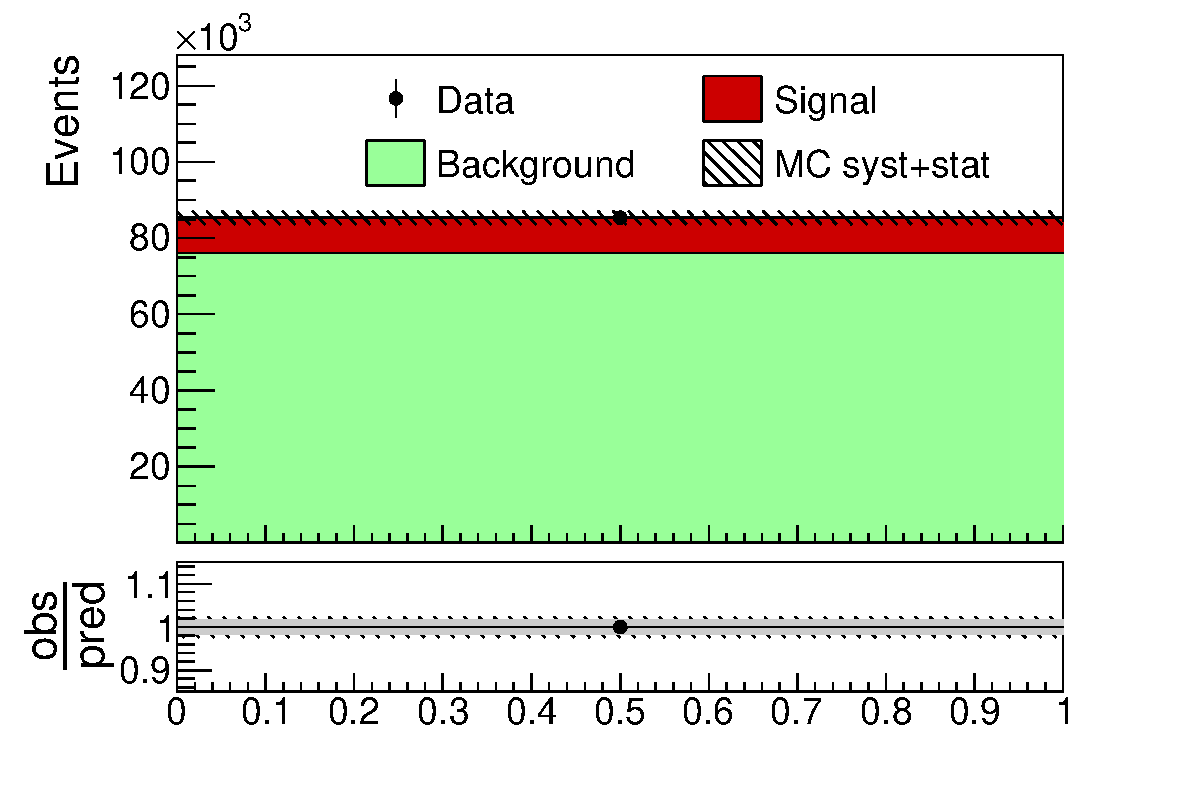
\includegraphics{Results/Figures/FitPlots/emu/total_0,0_b_jets_step_8_postfit.pdf}}
    \resizebox{0.32 \textwidth}{!}{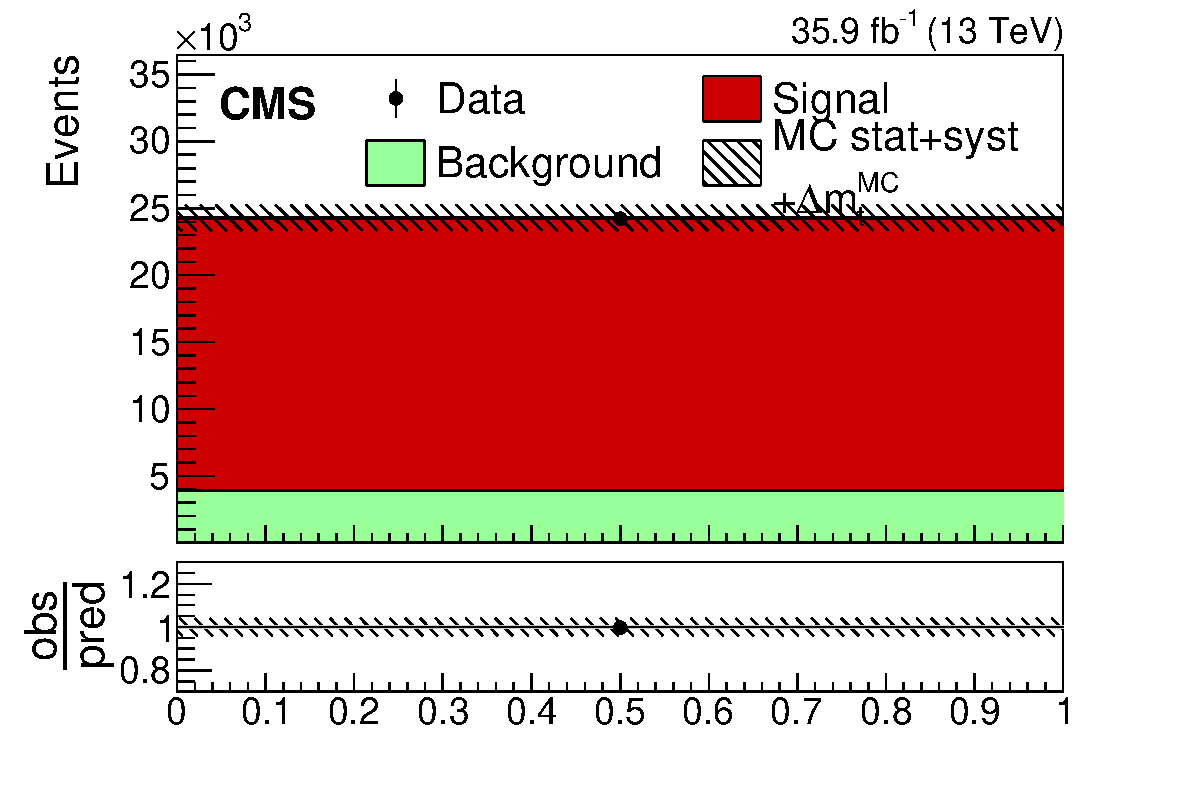
\includegraphics{Results/Figures/FitPlots/emu/total_1,0_b_jets_step_8_postfit.pdf}}
    \resizebox{0.32 \textwidth}{!}{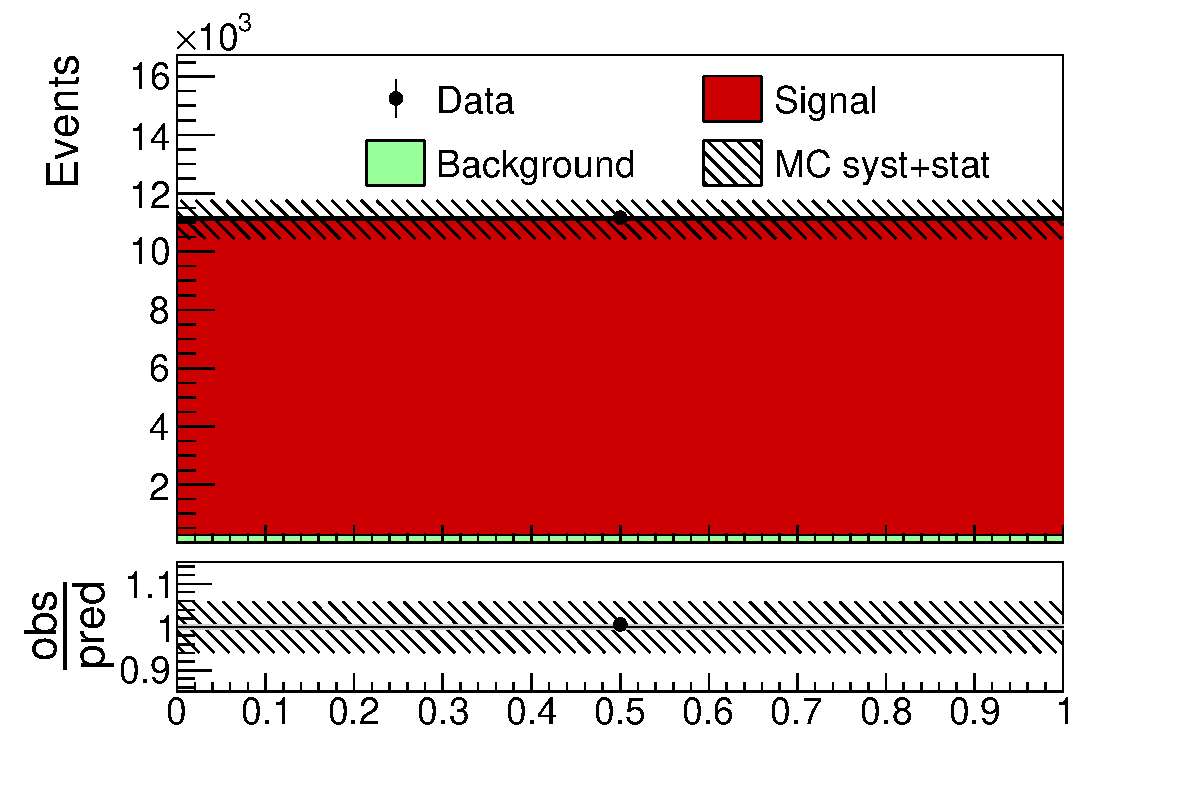
\includegraphics{Results/Figures/FitPlots/emu/total_2,0_b_jets_step_8_postfit.pdf}}

    \resizebox{0.32 \textwidth}{!}{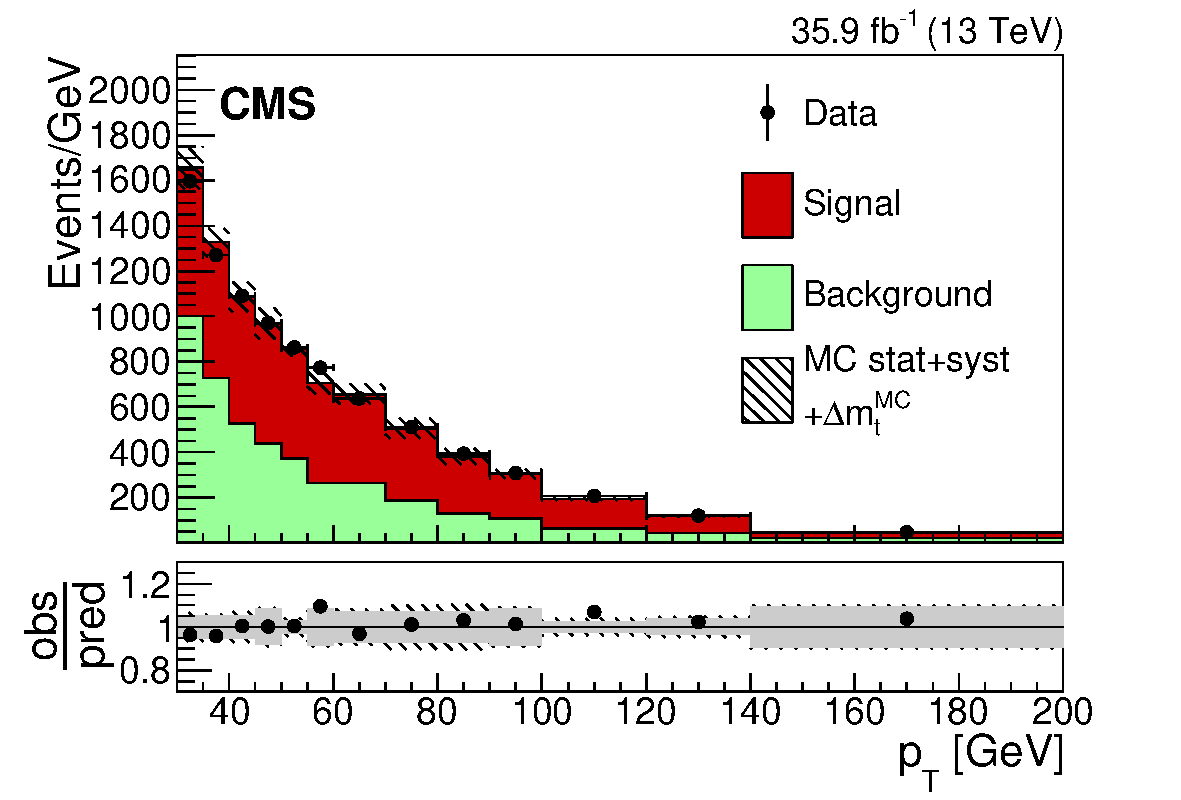
\includegraphics{Results/Figures/FitPlots/emu/lead_jet_pt_0,1_b_jets_step_8_postfit.pdf}}
    \resizebox{0.32 \textwidth}{!}{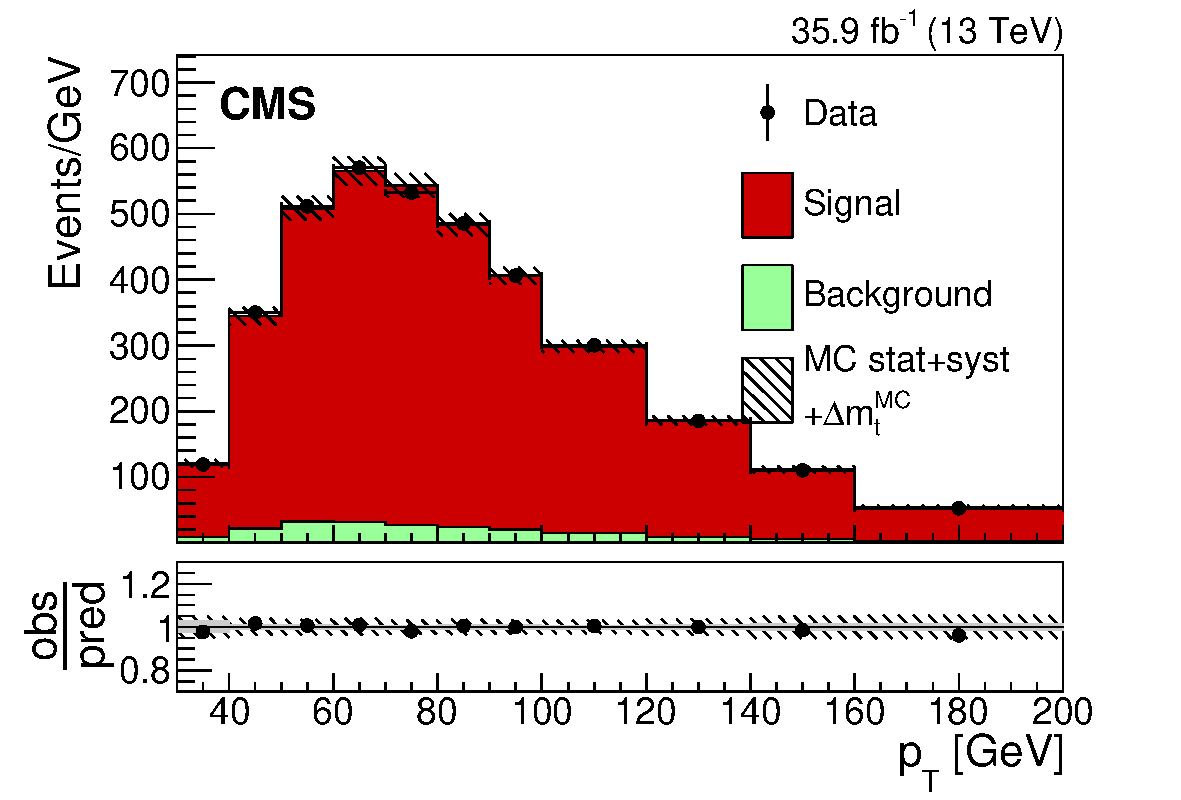
\includegraphics{Results/Figures/FitPlots/emu/lead_jet_pt_1,1_b_jets_step_8_postfit.pdf}}
    \resizebox{0.32 \textwidth}{!}{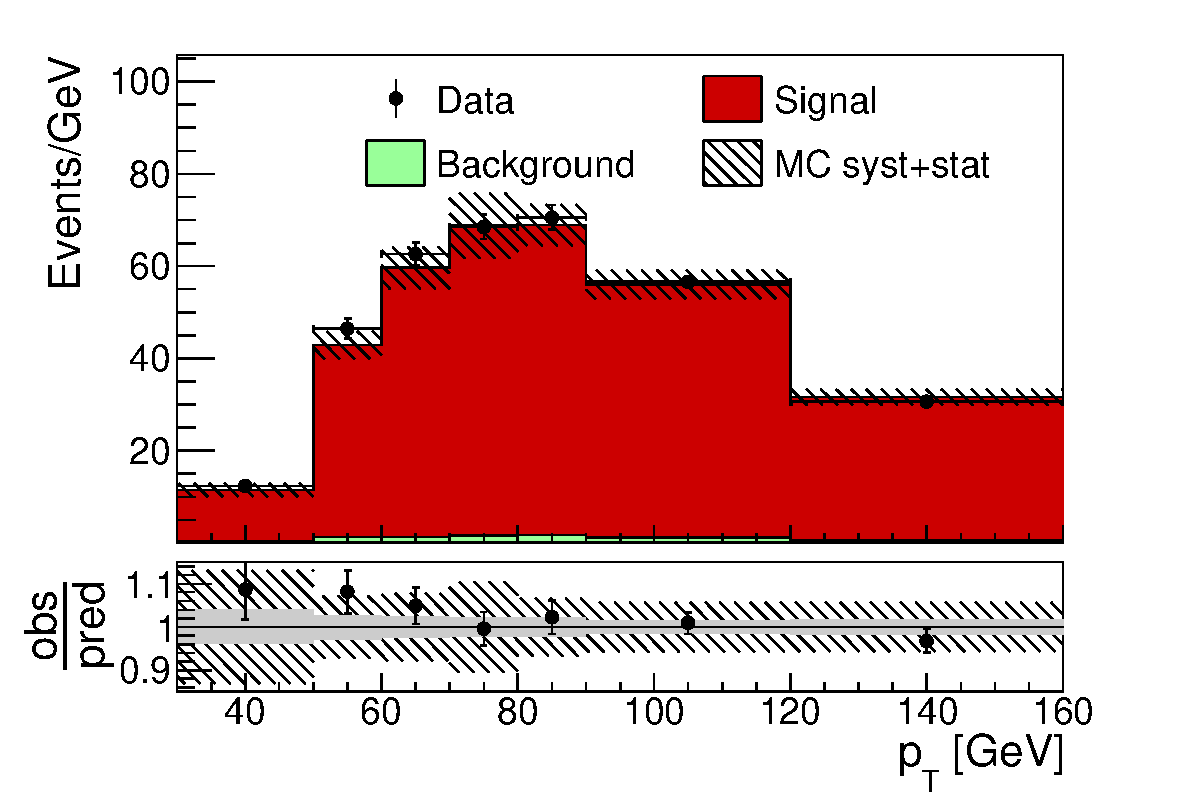
\includegraphics{Results/Figures/FitPlots/emu/lead_jet_pt_2,1_b_jets_step_8_postfit.pdf}}

    \resizebox{0.32 \textwidth}{!}{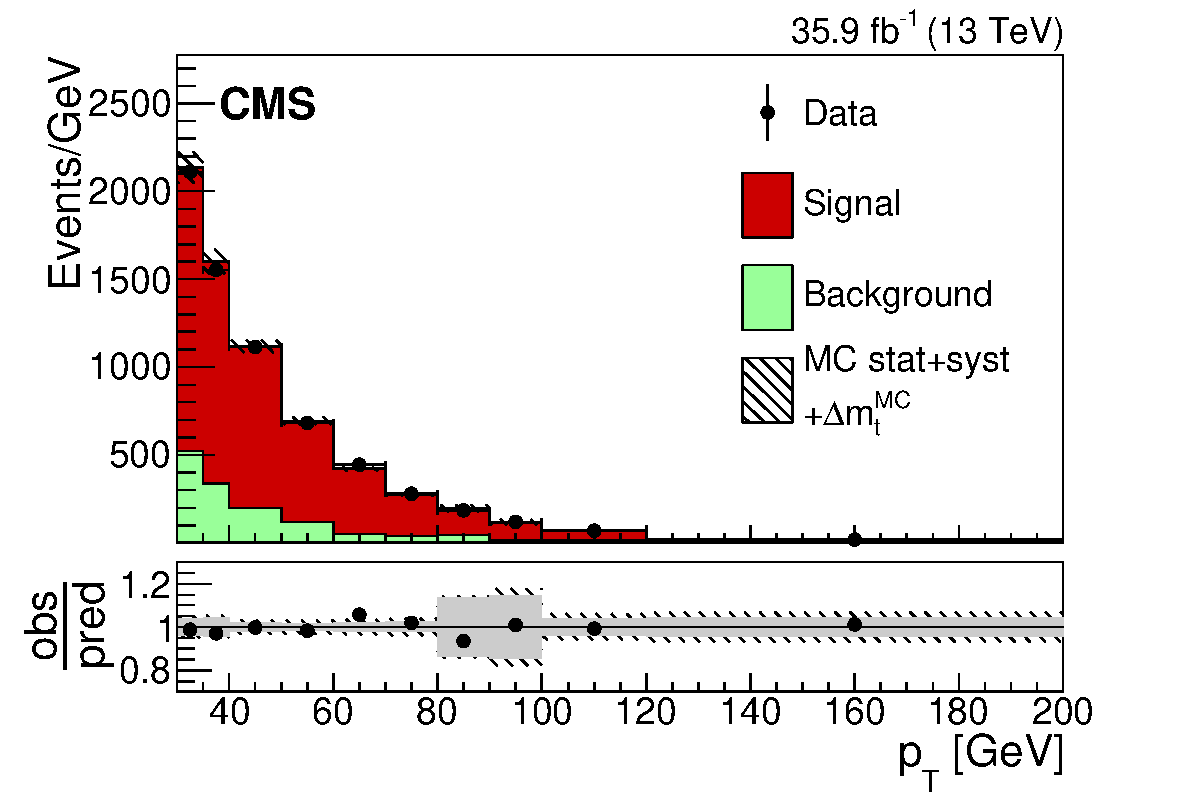
\includegraphics{Results/Figures/FitPlots/emu/second_jet_pt_0,2_b_jets_step_8_postfit.pdf}}
    \resizebox{0.32 \textwidth}{!}{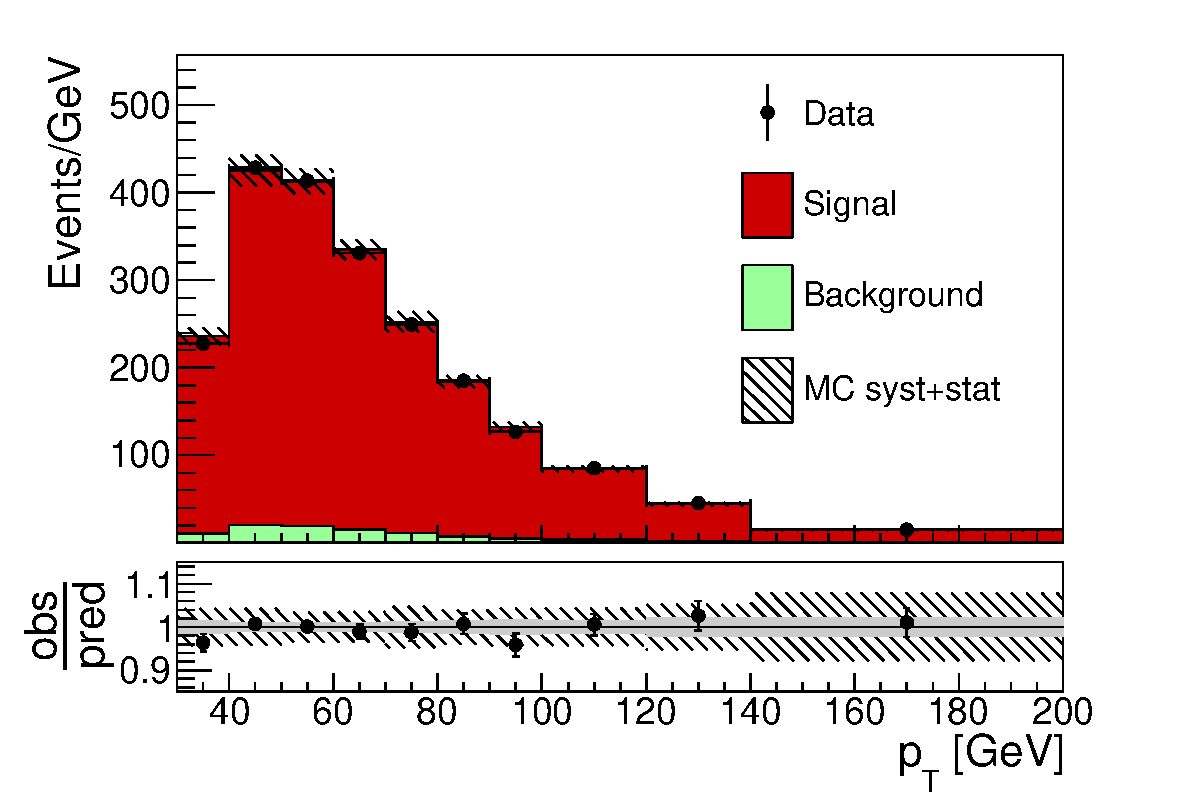
\includegraphics{Results/Figures/FitPlots/emu/second_jet_pt_1,2_b_jets_step_8_postfit.pdf}}
    \resizebox{0.32 \textwidth}{!}{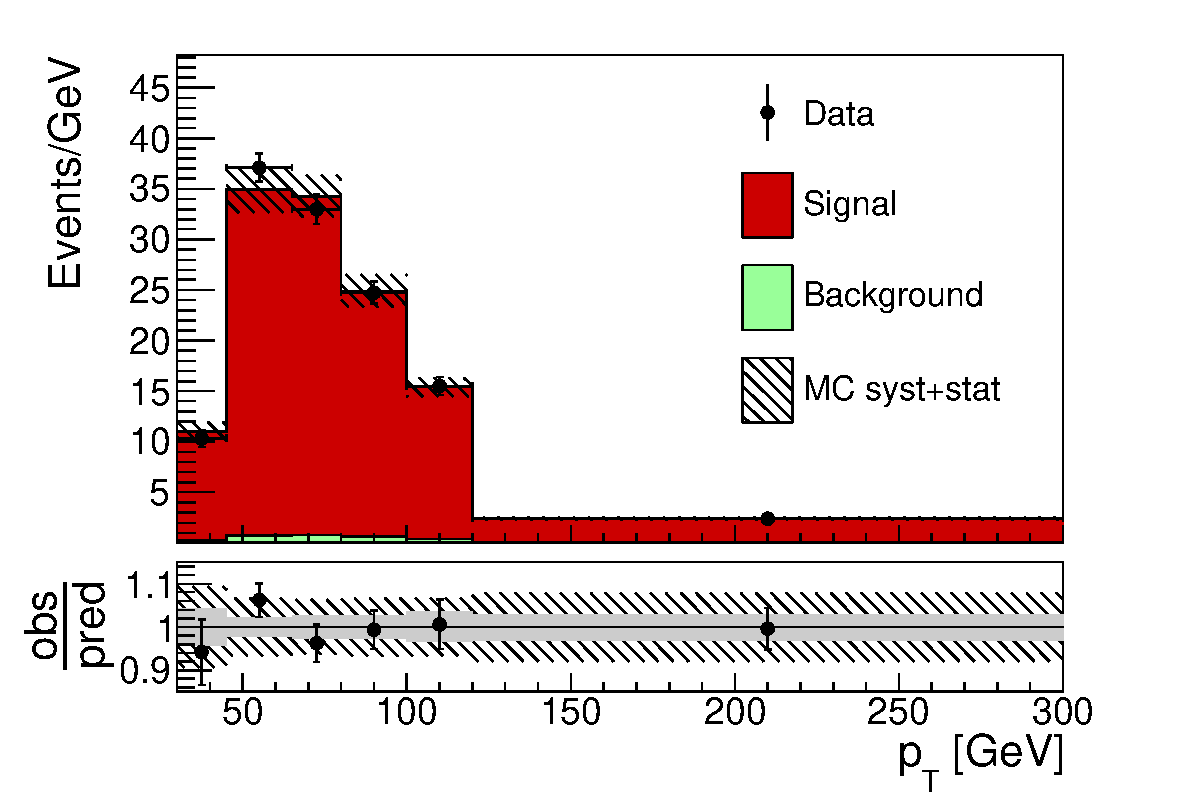
\includegraphics{Results/Figures/FitPlots/emu/second_jet_pt_2,2_b_jets_step_8_postfit.pdf}}    

    \resizebox{0.32 \textwidth}{!}{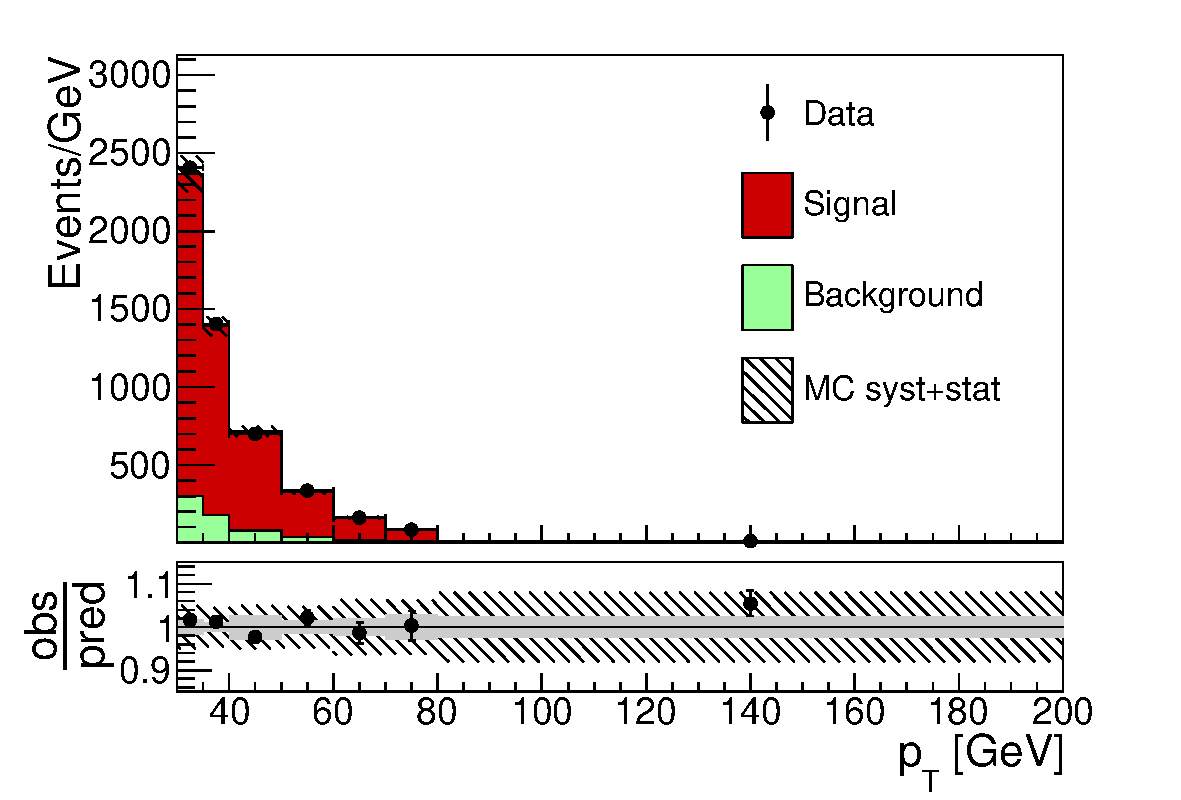
\includegraphics{Results/Figures/FitPlots/emu/third_jet_pt_0,3_b_jets_step_8_postfit.pdf}}
    \resizebox{0.32 \textwidth}{!}{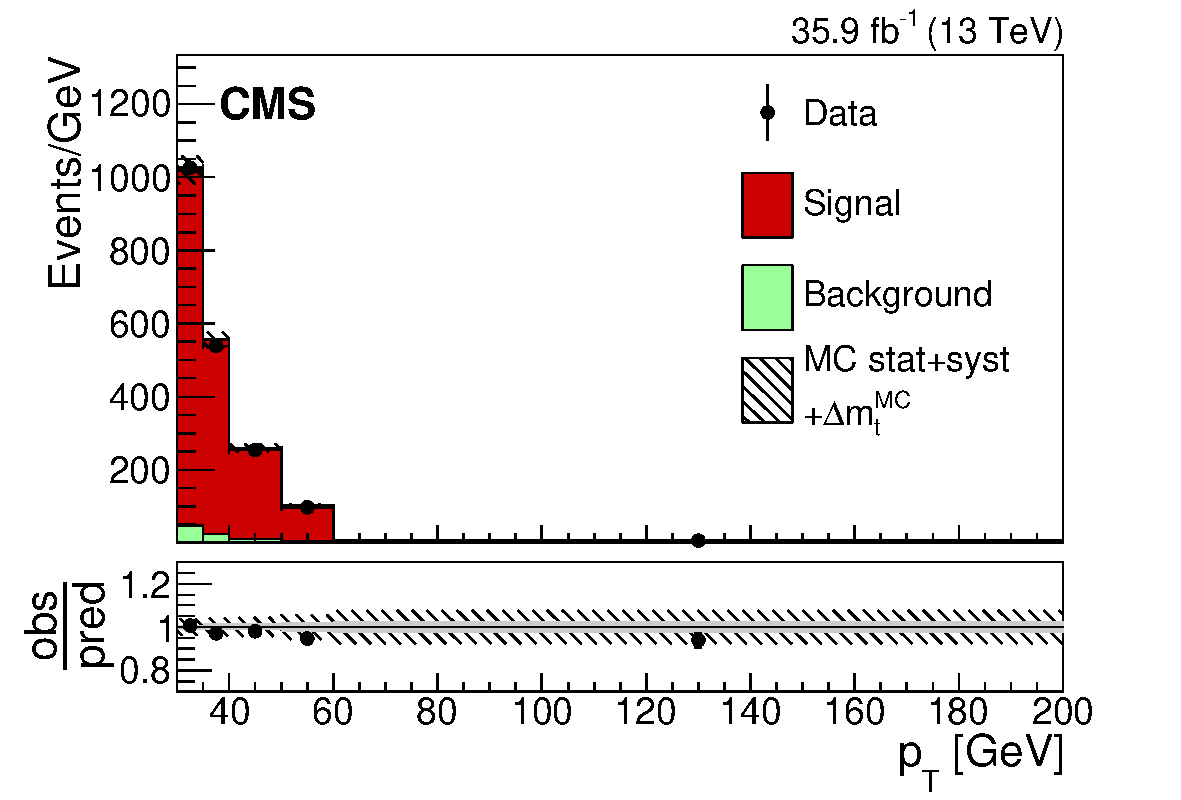
\includegraphics{Results/Figures/FitPlots/emu/third_jet_pt_1,3_b_jets_step_8_postfit.pdf}}
    \resizebox{0.32 \textwidth}{!}{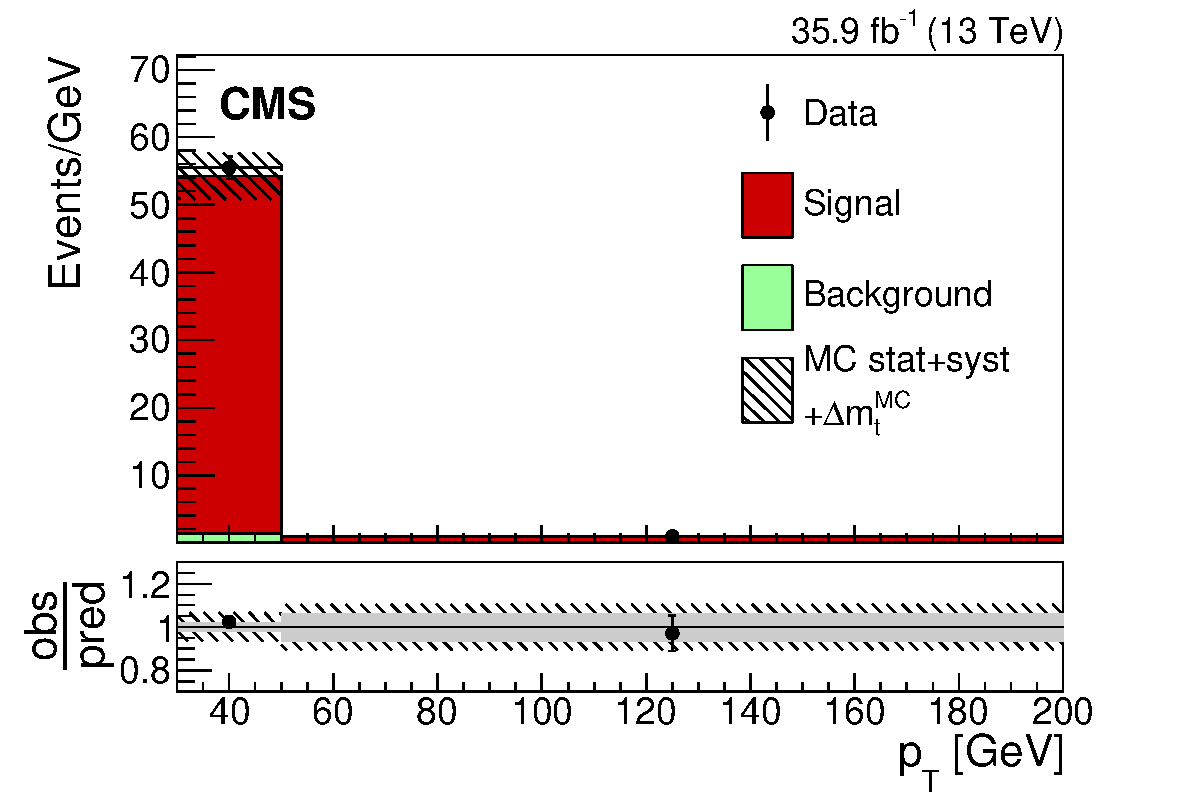
\includegraphics{Results/Figures/FitPlots/emu/third_jet_pt_2,3_b_jets_step_8_postfit.pdf}}   

\caption{Fitted Distributions (\emu channel) for events with zero as well as three or
  more b-tagged jets (left column): Total event yield for zero (top) and the trailing jet pt for one (second from top),
  two (second from bottom) or three or more (bottom) additional jets. The same for events with one
  b-tagged jet (middle column) and two b-tagged jets (right column) are
  shown below.   
  The hatched bands correspond to the total uncertainty on the sum of
  the predicted yields. The ratios of data to the sum of the
  predicted yields are shown at the bottom of each plot. Here, the solid
  gray band represents the contribution of the statistical uncertainty.   
       \label{fig:lh_emu_postfitdistr8}}
  \end{center}
\end{figure}

\begin{figure}[htbp!]
  \begin{center}

    \resizebox{0.32 \textwidth}{!}{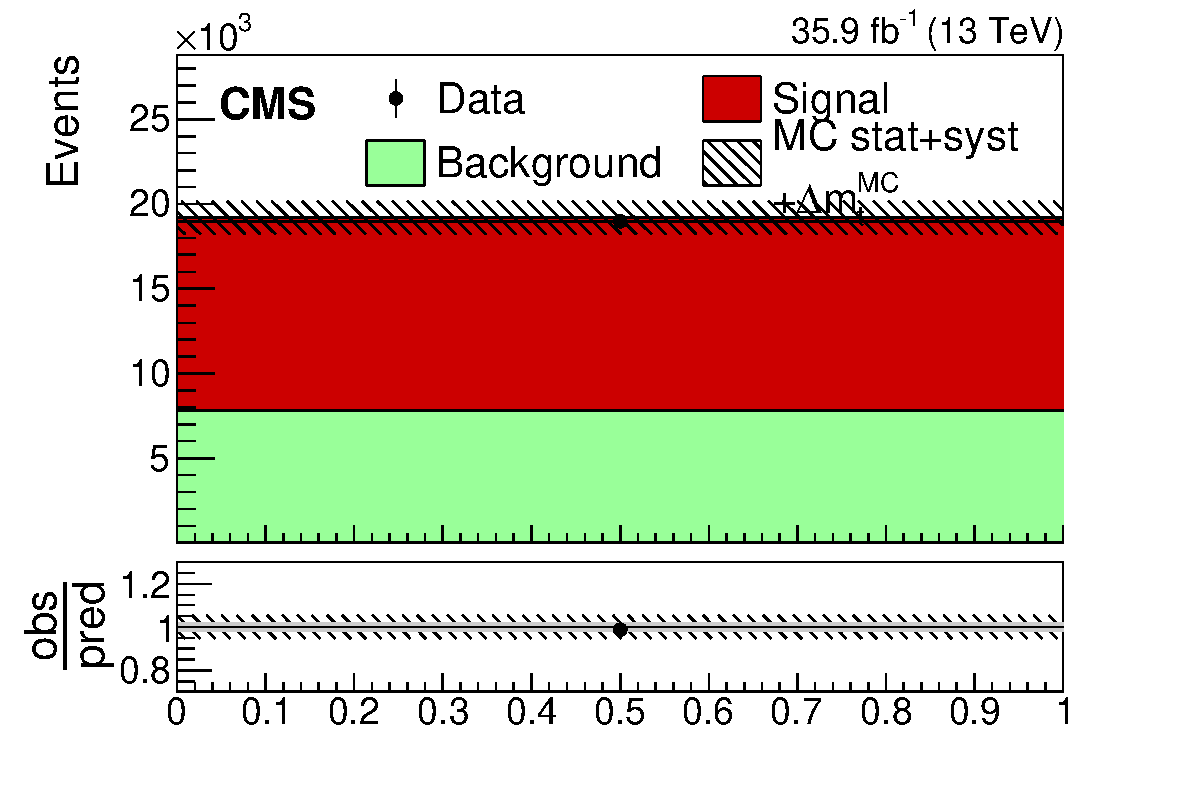
\includegraphics{Results/Figures/FitPlots/mumu/total_1,0_b_jets_step_8_postfit.pdf}}
    \resizebox{0.32 \textwidth}{!}{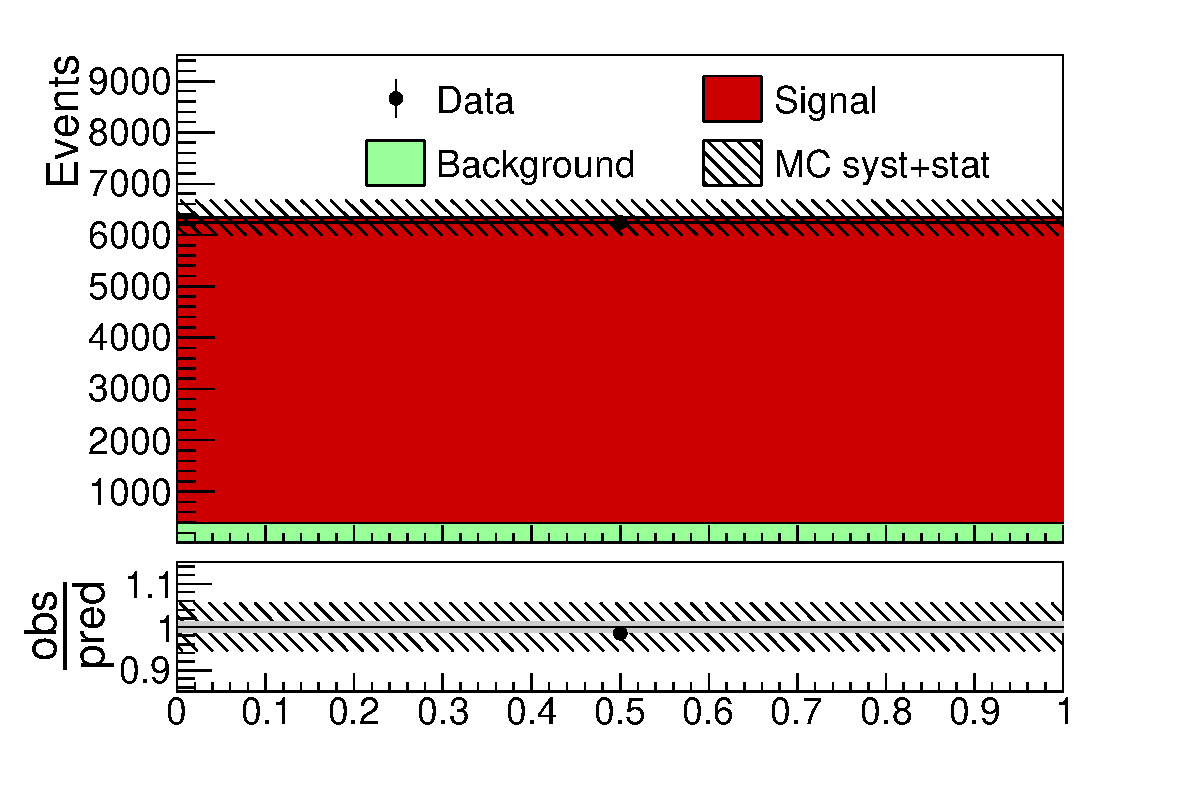
\includegraphics{Results/Figures/FitPlots/mumu/total_2,0_b_jets_step_8_postfit.pdf}}\\


    \resizebox{0.32 \textwidth}{!}{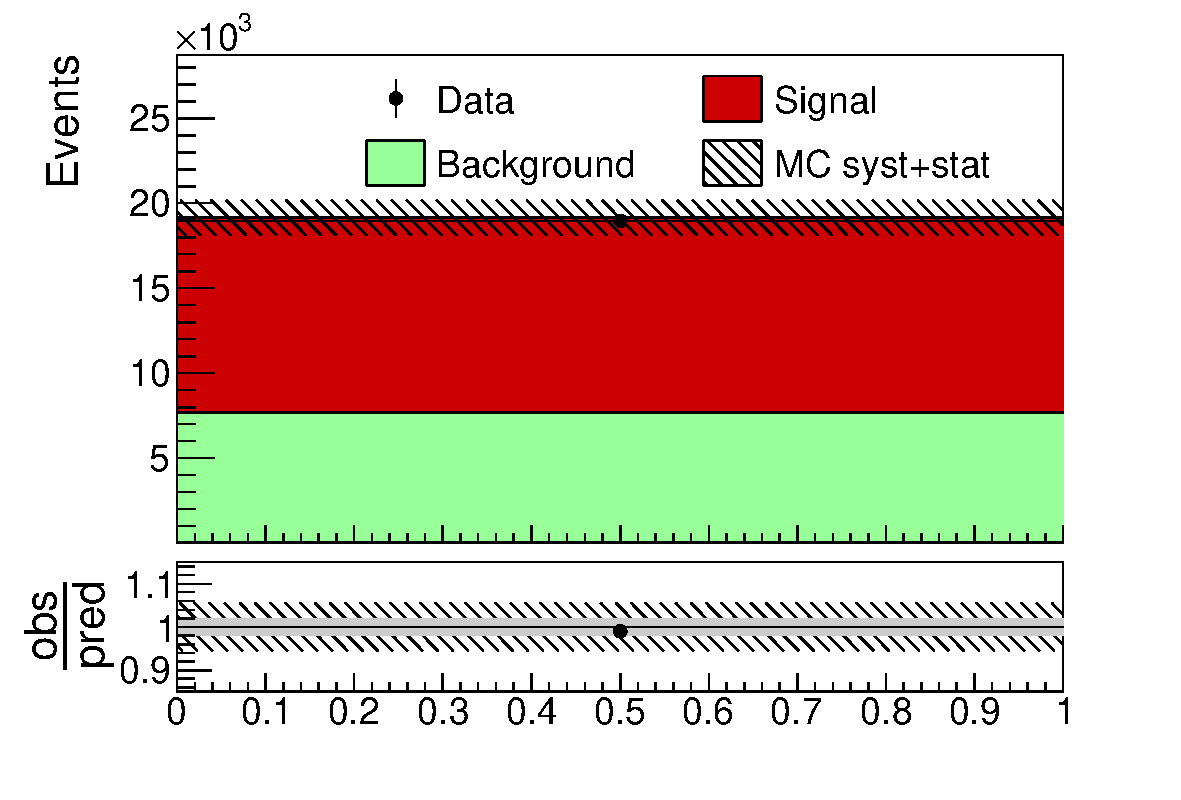
\includegraphics{Results/Figures/FitPlots/mumu/total_1,1_b_jets_step_8_postfit.pdf}}
    \resizebox{0.32 \textwidth}{!}{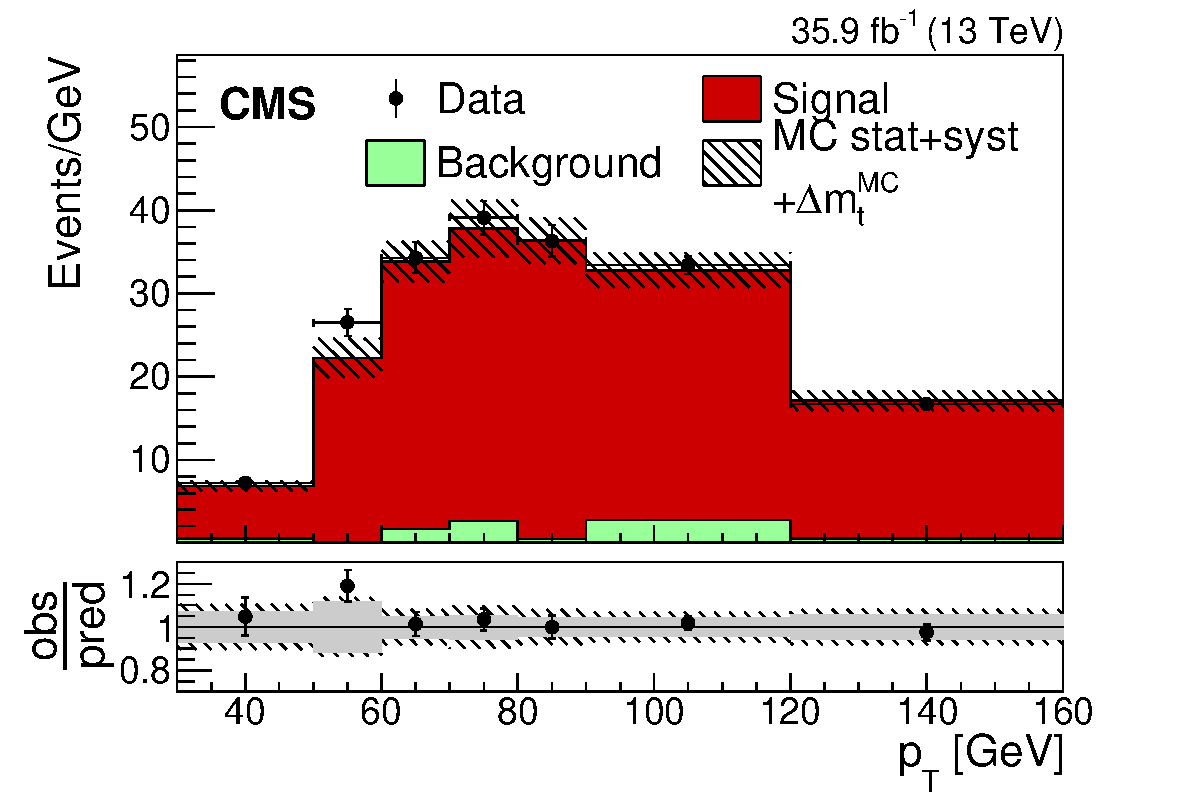
\includegraphics{Results/Figures/FitPlots/mumu/lead_jet_pt_2,1_b_jets_step_8_postfit.pdf}}\\


    \resizebox{0.32 \textwidth}{!}{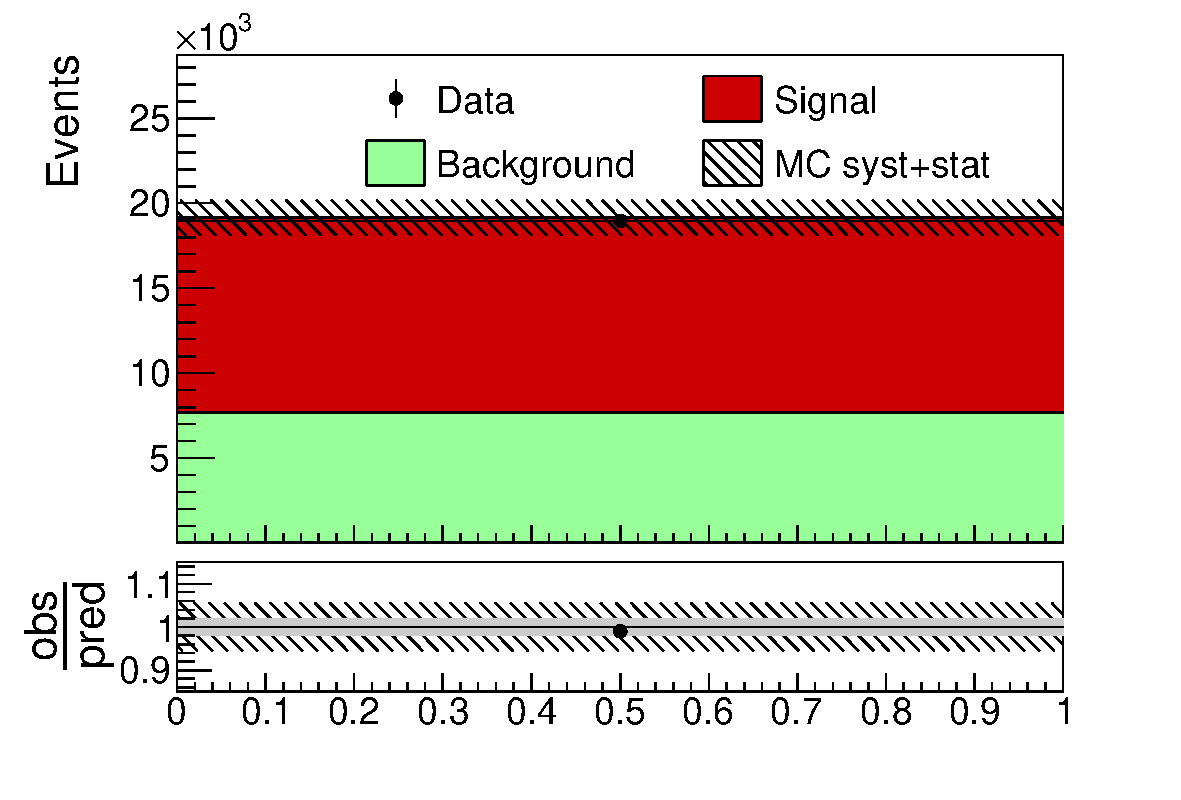
\includegraphics{Results/Figures/FitPlots/mumu/total_1,2_b_jets_step_8_postfit.pdf}}
    \resizebox{0.32 \textwidth}{!}{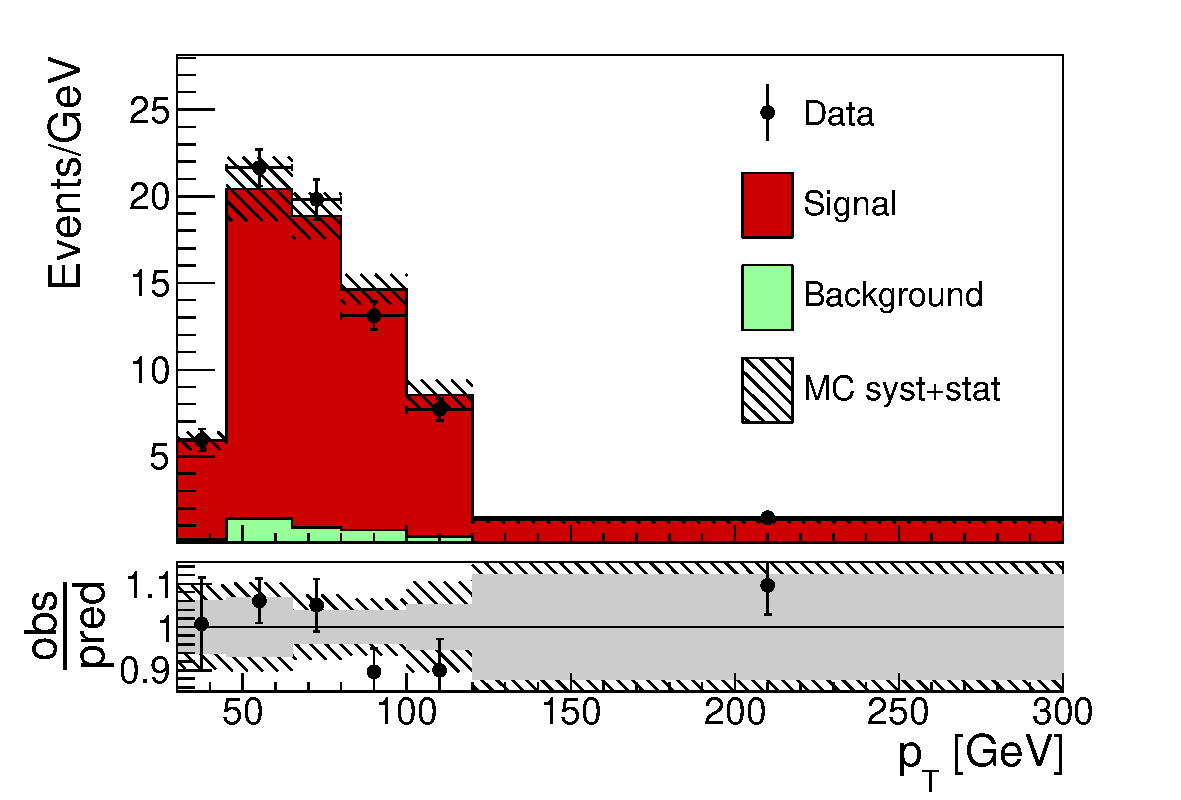
\includegraphics{Results/Figures/FitPlots/mumu/second_jet_pt_2,2_b_jets_step_8_postfit.pdf}}  \\  


    \resizebox{0.32 \textwidth}{!}{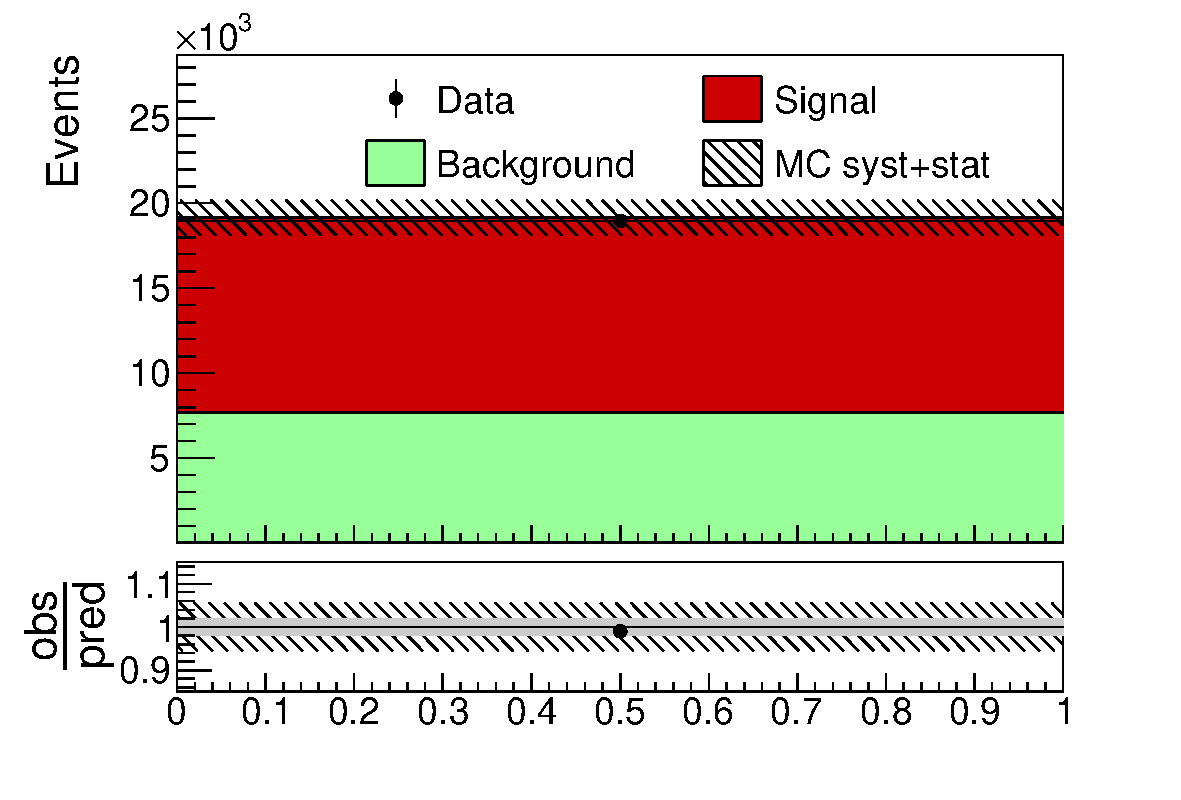
\includegraphics{Results/Figures/FitPlots/mumu/total_1,3_b_jets_step_8_postfit.pdf}}
    \resizebox{0.32 \textwidth}{!}{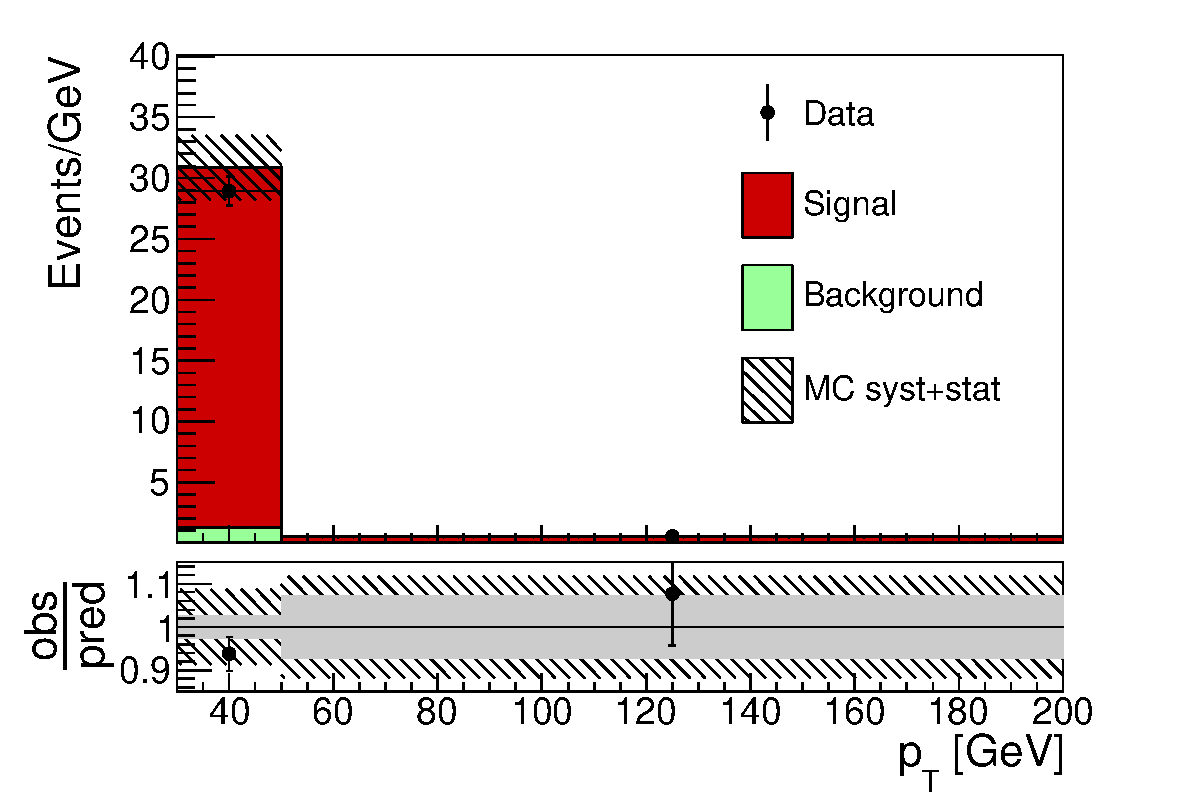
\includegraphics{Results/Figures/FitPlots/mumu/third_jet_pt_2,3_b_jets_step_8_postfit.pdf}}   

\caption{Fitted distributions (\mumu channel): 
  The left column shows events with one b-tagged jet and the total event yield for events with zero (top), one (second from top)
  two (second from bottom) or three or more additional jets (bottom).
  The right column shows events with two b-tagged jets and the total yield for events with zero additional jets (top),
  the trailing jet pt for one (second from top),
  two (second from bottom) or three or more (bottom) additional jets.
  The hatched bands correspond to the total uncertainty on the sum of
  the predicted yields. The ratios of data to the sum of the
  predicted yields are shown at the bottom of each plot. Here, the solid
  gray band represents the contribution of the statistical uncertainty.  
       \label{fig:lh_mumu_postfitdistr8}}
  \end{center}
\end{figure}

\begin{figure}[htbp!]
  \begin{center}
    \resizebox{0.32 \textwidth}{!}{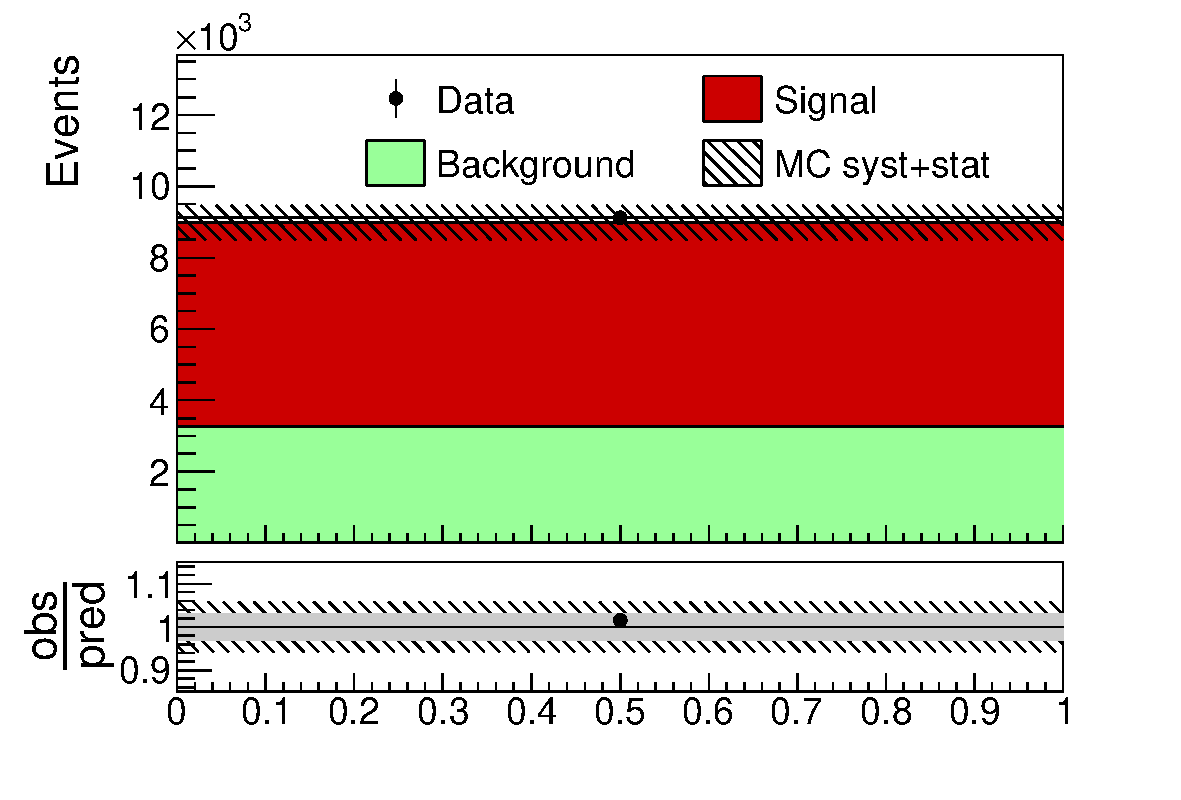
\includegraphics{Results/Figures/FitPlots/ee/total_1,0_b_jets_step_8_postfit.pdf}}
    \resizebox{0.32 \textwidth}{!}{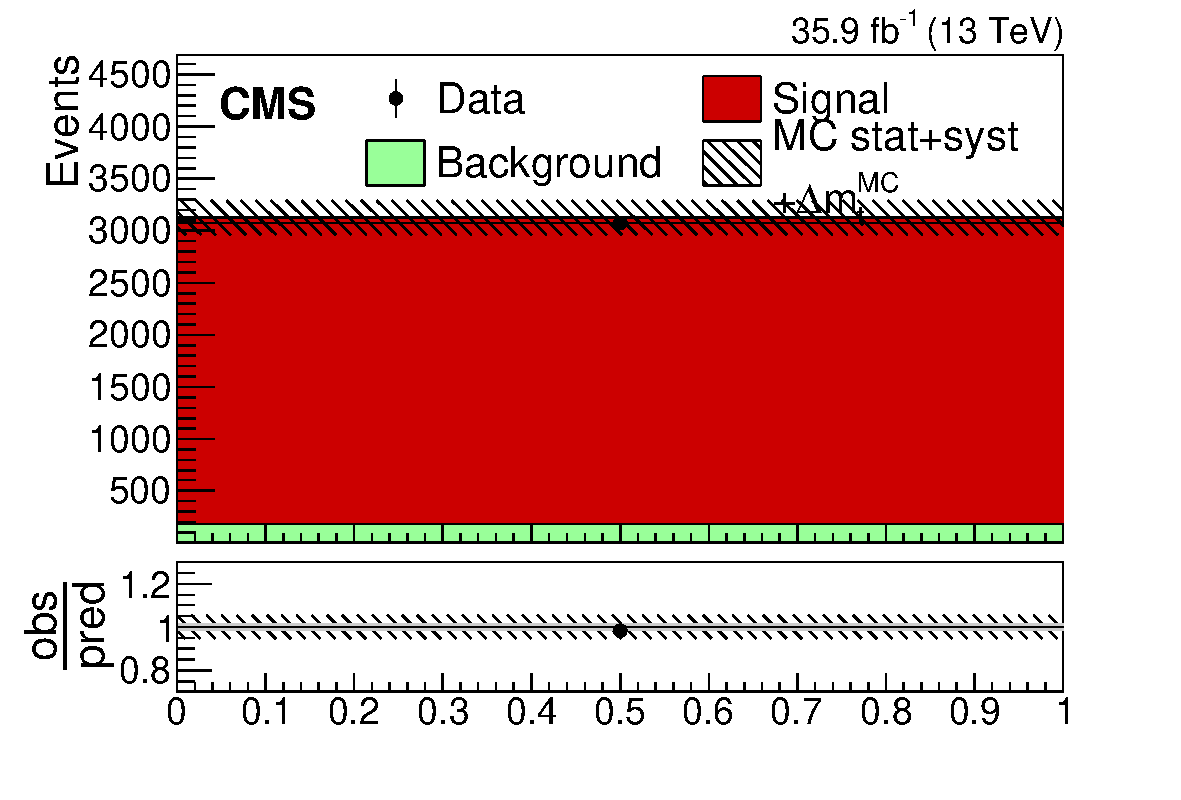
\includegraphics{Results/Figures/FitPlots/ee/total_2,0_b_jets_step_8_postfit.pdf}}\\

    \resizebox{0.32 \textwidth}{!}{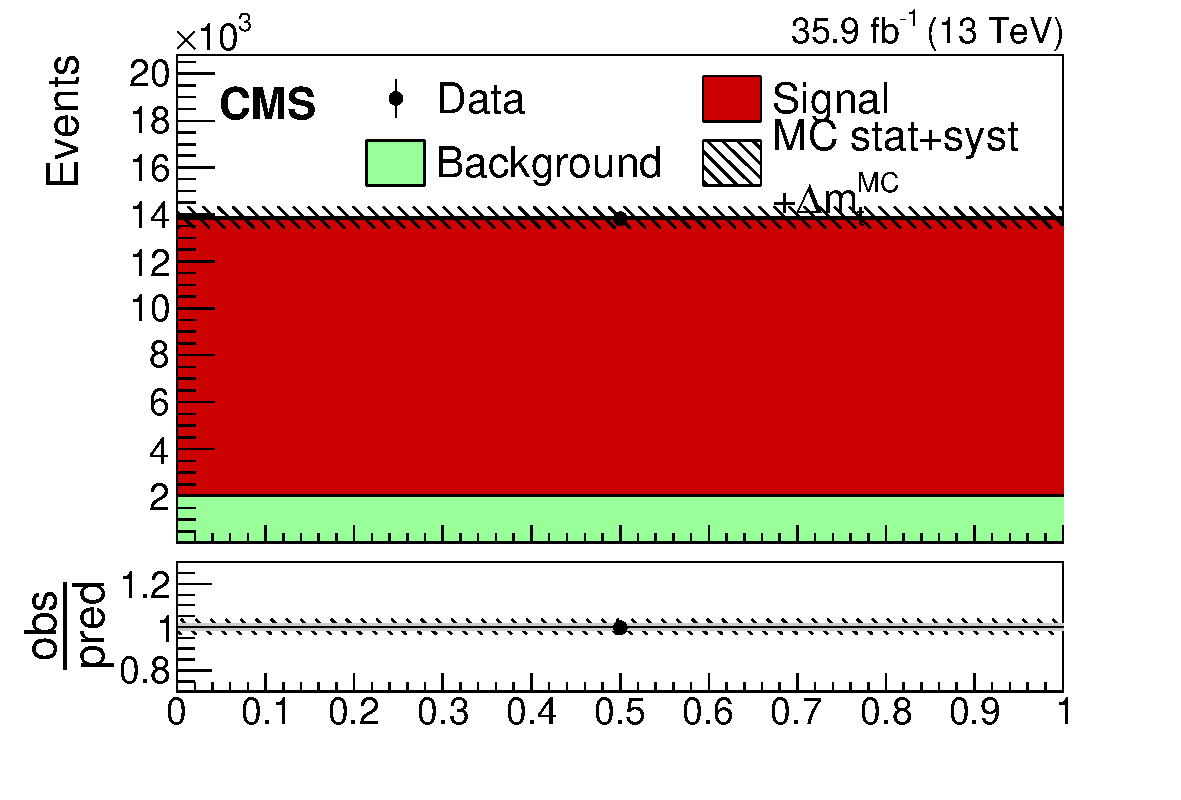
\includegraphics{Results/Figures/FitPlots/ee/total_1,1_b_jets_step_8_postfit.pdf}}
    \resizebox{0.32 \textwidth}{!}{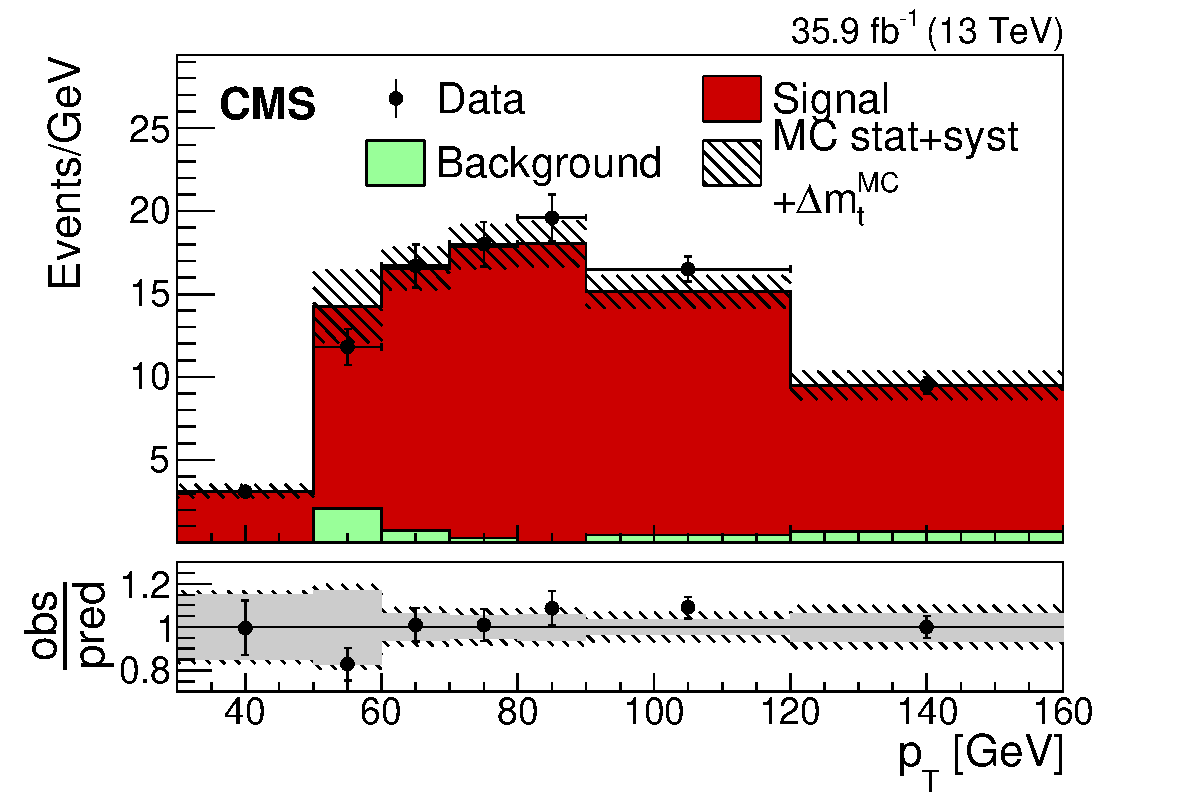
\includegraphics{Results/Figures/FitPlots/ee/lead_jet_pt_2,1_b_jets_step_8_postfit.pdf}}\\

    \resizebox{0.32 \textwidth}{!}{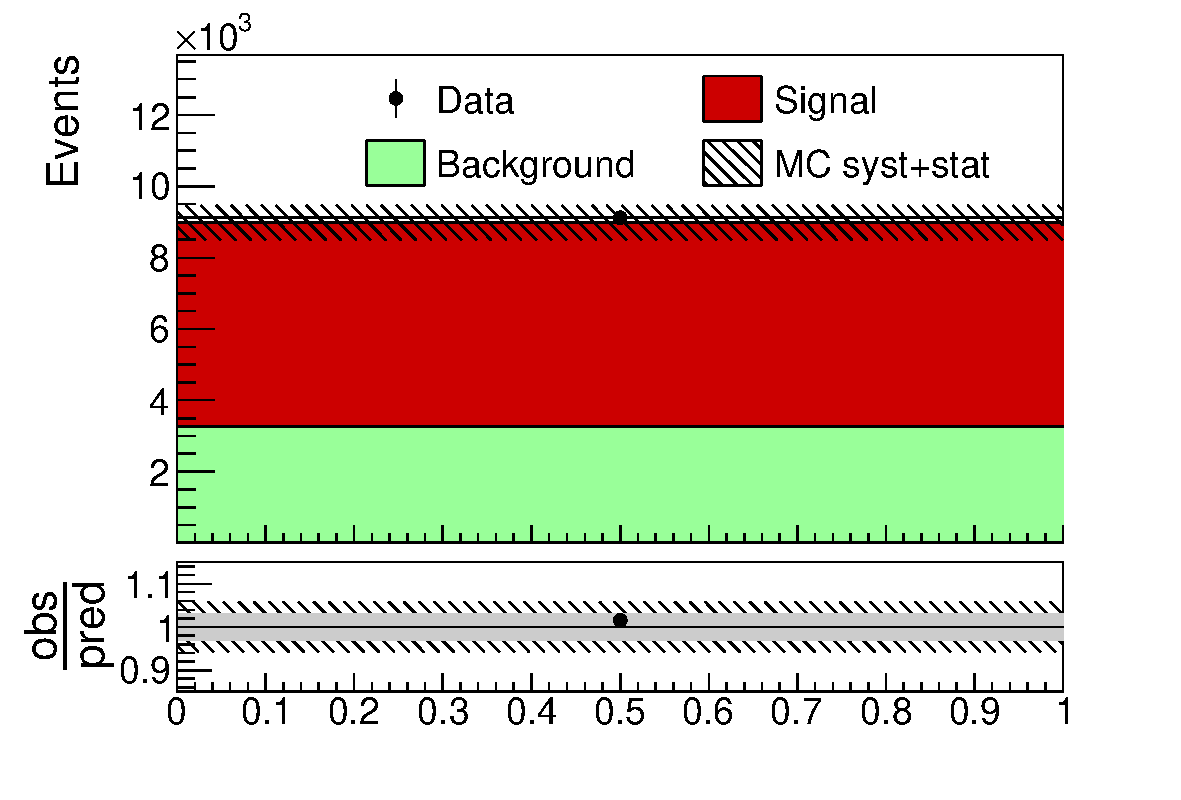
\includegraphics{Results/Figures/FitPlots/ee/total_1,2_b_jets_step_8_postfit.pdf}}
    \resizebox{0.32 \textwidth}{!}{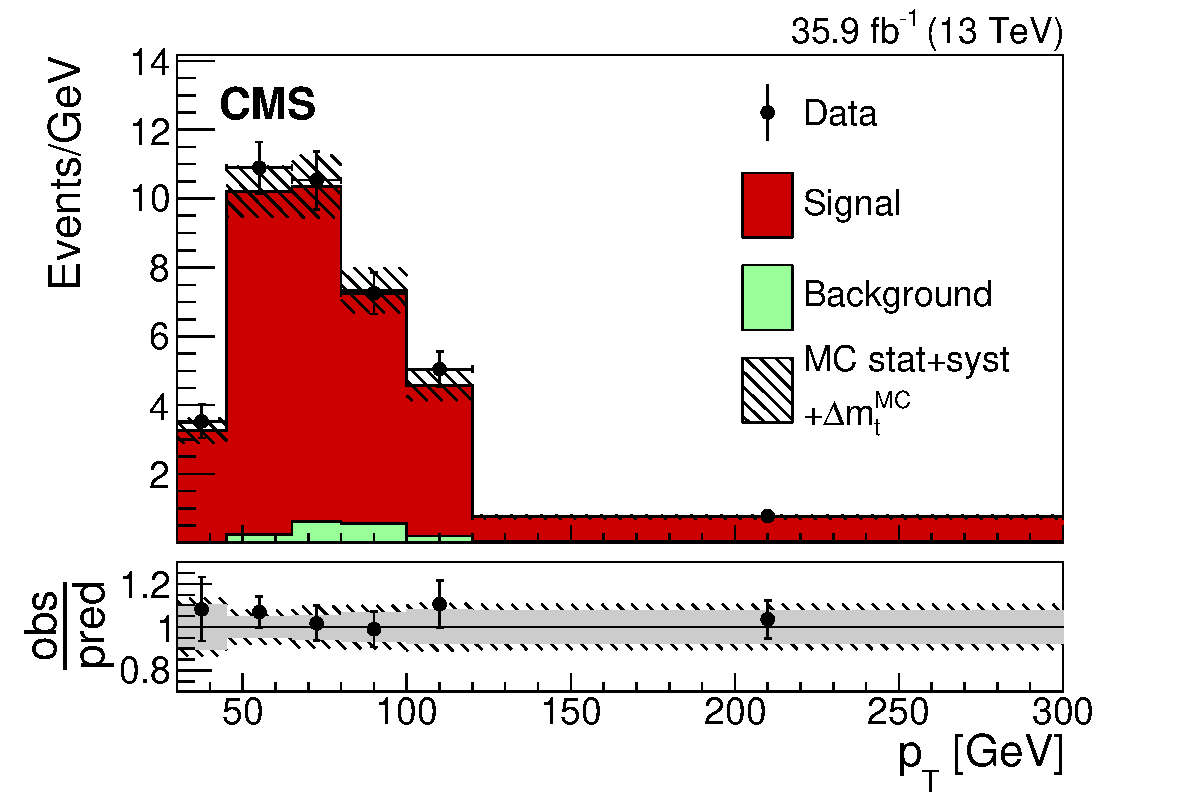
\includegraphics{Results/Figures/FitPlots/ee/second_jet_pt_2,2_b_jets_step_8_postfit.pdf}} \\   

    \resizebox{0.32 \textwidth}{!}{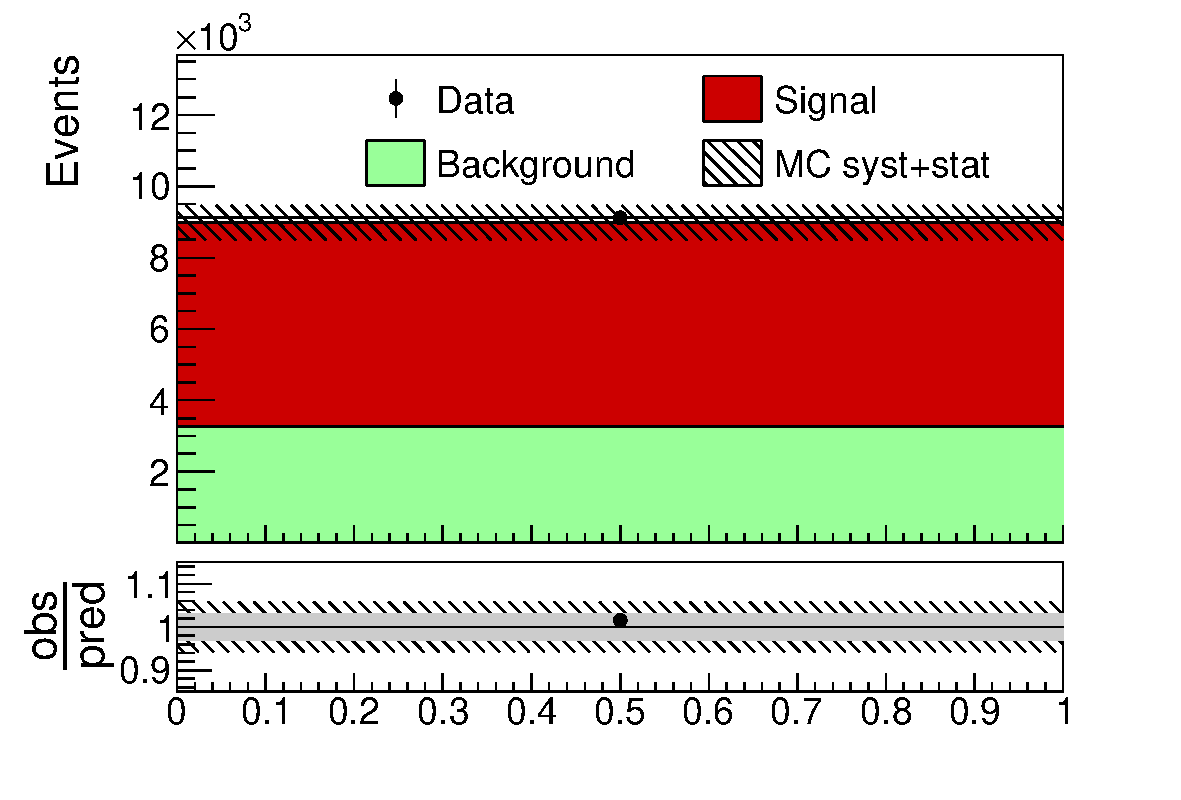
\includegraphics{Results/Figures/FitPlots/ee/total_1,3_b_jets_step_8_postfit.pdf}}
    \resizebox{0.32 \textwidth}{!}{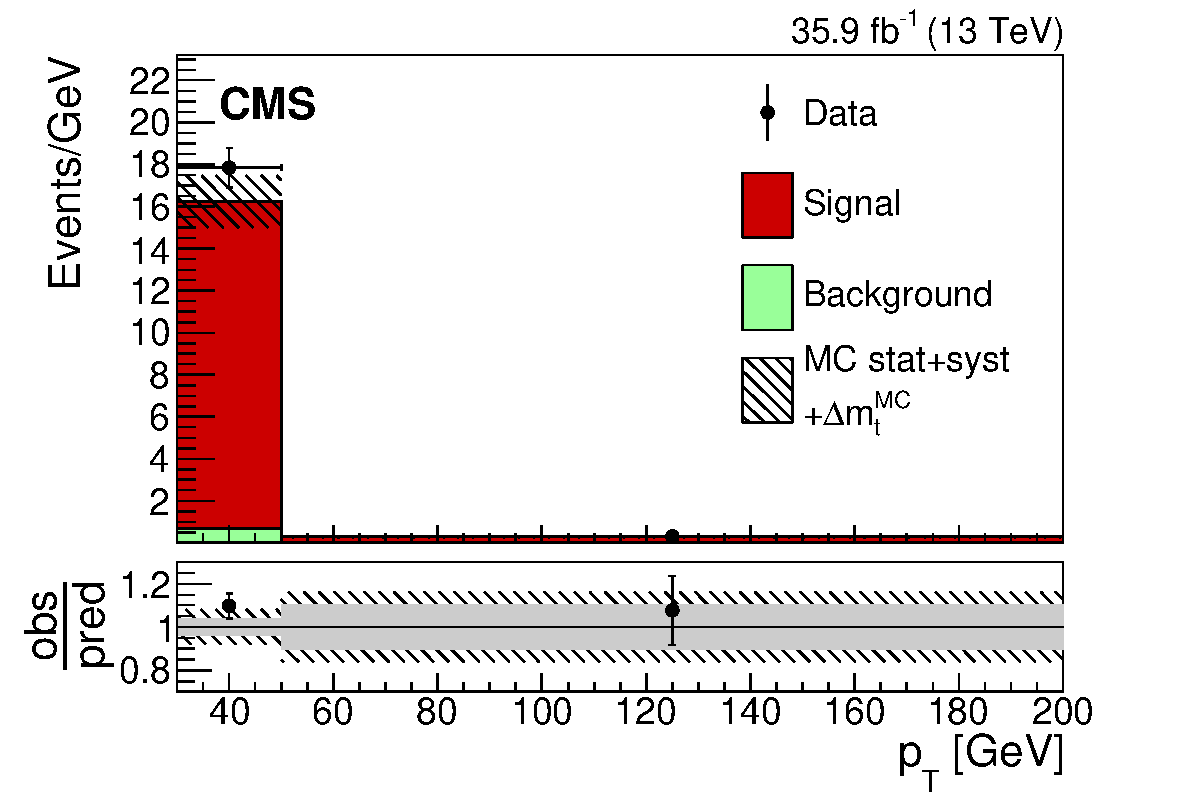
\includegraphics{Results/Figures/FitPlots/ee/third_jet_pt_2,3_b_jets_step_8_postfit.pdf}}   

\caption{Fitted distributions (\ee channel): 
  The left column shows events with one b-tagged jet and the total event yield for events with zero (top), one (second from top)
  two (second from bottom) or three or more additional jets (bottom).
  The right column shows events with two b-tagged jets and the total yield for events with zero additional jets (top),
  the trailing jet pt for one (second from top),
  two (second from bottom) or three or more (bottom) additional jets.
  The hatched bands correspond to the total uncertainty on the sum of
  the predicted yields. The ratios of data to the sum of the
  predicted yields are shown at the bottom of each plot. Here, the solid
  gray band represents the contribution of the statistical uncertainty.  
       \label{fig:lh_ee_postfitdistr8}}
  \end{center}
\end{figure}

The plots show that simulation agrees with the data after applying the fitted parameters.
The agreement can be expected and shows that the fit succesfully scales simulation to data.
The simulation is able to model the data within its uncertainties.
The plotted uncertainties are smaller compared to the plots showing the non-constrained uncertainties in Figure \ref{fig:xsec_emu_inputdistr},\ref{fig:xsec_mumu_inputdistr} and \ref{fig:xsec_ee_inputdistr}.
This reduction of the uncertainty roughly corresponds to the statistical uncertainty of the data.



\section{Breakdown of systematic uncertainties}
\label{sec:results_uncert}

As described in Section \ref{sec:xsec_stat} the results of the fit include the \ttbar cross section value as well as the results for the fitted nuisance parameters.
For the nuisance parameters a fitted value (also called pull) of $0$ stands for the nominal result, while a value of $\pm 1$ stands for the $\pm 1 \; \sigma$ variation.
The impact of each of the nuisance parameters on the cross section is estimated by fixing one nuisance parameter to the nominal value and repeating the fit.
The reduction in the resulting uncertainty on the cross section is then considered as the contribution of that single uncertainty. This calculation does not consider correlations between multiple uncertainties,
so the quadratic sum of the contributions of all uncertainties does not correspond to the total uncertainty.

Table \ref{tab:lh_res_eightfull} shows the results for the pulls of the nuisance parameters, their constraints and the impact on the cross section.
It also shows the result for the cross section itself and for the extrapolation of the full to the visible phase space including the extrapolation of the relevant uncertainties.

\begin{longtable}{ l | c | c | c }%[htbp!]
%\center
\caption{Extracted cross sections with detailed
  list of uncertainties. Besides the contribution to the total
  uncertainty in \%, the fitted value of the nuisance parameter (pull), as well as the ratio of the estimated
  uncertainty over the uncertainty from a 1 $\sigma$ variation, called
  constr/$\sigma$, are shown. 
  \label{tab:lh_res_eightfull}}\\
\hline
Name & Pull & Constr / $\sigma$ & Contribution [\%] \\ 
\hline
\endfirsthead
\hline
Name & Pull & Constr / $\sigma$ & Contribution [\%] \\ 
\hline
\endhead
B-tag & 0.617 & 0.49 & ${0.456}$ \\
Mistag & 0.413 & 0.96 & ${0.129}$ \\
DY ME scale & -0.583 & 0.44 & ${0.118}$ \\
Electron energy resolution & -0.076 & 0.91 & ${-0.007}$ \\
Electron energy scale & -1.271 & 0.63 & ${-0.015}$ \\
Electron ID & 0.291 & 0.6 & ${-1.907}$ \\
Jet energy resolution & 1.096 & 0.81 & ${-0.008}$ \\
JES: MPF & 0.101 & 0.66 & ${0.002}$ \\
JES: Absolute Scale & -0.053 & 0.77 & ${0.019}$ \\
JES: Absolute Stat & 0.266 & 0.83 & ${-0.039}$ \\
JES\_Fragmentation & 0.203 & 0.63 & ${-0.038}$ \\
JES: Pileup Data/MC & -0.265 & 0.89 & ${-0.063}$ \\
JES: Pileup $p_T$ BB & 0.166 & 0.75 & ${-0.093}$ \\
JES\_PileUpPtEC1 & -0.12 & 0.65 & ${-0.046}$ \\
JES\_PileUpPtRef & 0.28 & 0.56 & ${-0.084}$ \\
JES\_RelativeBal & -0.709 & 0.52 & ${0.143}$ \\
JES: Intercalibration & 0.068 & 0.66 & ${-0.001}$ \\
JES: Relative JER EC1 & -0.074 & 1.03 & ${0.008}$ \\
JES: Relative $p_T$ BB & -0.025 & 0.87 & ${0.019}$ \\
JES: Relative $p_T$ EC1 & -0.012 & 0.91 & ${-0.049}$ \\
JES\_RelativeStatEC & 0.296 & 0.73 & ${-0.026}$ \\
JES\_RelativeStatFSR & -0.085 & 1.07 & ${0.033}$ \\
JES: Single pion ECAL & 0.264 & 0.6 & ${-0.060}$ \\
JES: Single pion HCAL & 0.171 & 0.63 & ${-0.026}$ \\
JES\_TimePtEta & 0.255 & 0.68 & ${-0.019}$ \\
Muon energy scale & 0.114 & 0.99 & ${0.043}$ \\
Muon ID & -0.343 & 0.84 & ${-2.021}$ \\
Pile-up & 0.511 & 0.82 & ${0.312}$ \\
top mass & 0 & 0 & ${0.000}$ \\
Top $p_{T}$ & 1 & 0.74 & ${-0.001}$ \\
Trigger & -0.022 & 0.99 & ${-0.645}$ \\
B-hadron BR & 0.093 & 0.72 & ${0.075}$ \\
TT\_CRERD & 0 & 0.69 & ${0.000}$ \\
TT\_CRGLUON & 0.184 & 0.17 & ${0.006}$ \\
TT\_CRQCD & 0.105 & 0.12 & ${0.139}$ \\
fragm. Peterson & 0.521 & 0.41 & ${0.302}$ \\
fragmentation & -0.768 & 0.58 & ${-0.694}$ \\
$t\bar{t}$/tW FSR scale & -0.201 & 0.17 & ${0.560}$ \\
NLO generator & 0 & 0 & ${0.000}$ \\
$t\bar{t}$/tW ISR scale & 0.111 & 0.18 & ${-0.305}$ \\
ME/PS matching & -0.138 & 0.2 & ${0.148}$ \\
$t\bar{t}$ ME scale & 1 & 0.32 & ${0.000}$ \\
UE tune & 0.163 & 0.26 & ${0.180}$ \\
PDF10 & -0.065 & 0.84 & ${0.367}$ \\
PDF11 & -0.003 & 0.86 & ${0.139}$ \\
PDF12 & 0.022 & 0.86 & ${-0.209}$ \\
PDF13 & 0.21 & 0.85 & ${0.155}$ \\
PDF14 & 0.06 & 0.87 & ${-0.082}$ \\
PDF15 & 0.061 & 0.83 & ${-0.051}$ \\
PDF16 & 0.004 & 0.86 & ${0.061}$ \\
PDF17 & -0.043 & 0.85 & ${-0.150}$ \\
PDF18 & -0.228 & 0.85 & ${0.021}$ \\
PDF19 & -0.106 & 0.82 & ${0.257}$ \\
PDF1 & -0.018 & 0.88 & ${-0.037}$ \\
PDF20 & 0.002 & 0.83 & ${0.098}$ \\
PDF21 & -0.115 & 0.86 & ${-0.173}$ \\
PDF22 & -0.239 & 0.85 & ${-0.223}$ \\
PDF23 & 0.096 & 0.76 & ${-0.008}$ \\
PDF24 & 0.104 & 0.87 & ${0.137}$ \\
PDF25 & -0.083 & 0.83 & ${-0.020}$ \\
PDF26 & 0.013 & 0.83 & ${0.021}$ \\
PDF27 & -0.045 & 0.88 & ${0.092}$ \\
PDF28 & 0.035 & 0.85 & ${-0.011}$ \\
PDF2 & -0.241 & 0.97 & ${-0.047}$ \\
PDF3 & -0.005 & 0.86 & ${0.147}$ \\
PDF4 & -0.092 & 0.92 & ${0.071}$ \\
PDF5 & 0.085 & 0.8 & ${-0.329}$ \\
PDF6 & -0.006 & 0.87 & ${0.109}$ \\
PDF7 & 0.16 & 0.78 & ${-0.385}$ \\
PDF8 & 0.046 & 0.85 & ${-0.026}$ \\
PDF9 & -0.084 & 0.85 & ${-0.014}$ \\
JES: Flavor response & -0.335 & 0.63 & ${-0.076}$ \\
tW background & -0.422 & 0.46 & ${-0.815}$ \\
Diboson background & 0.849 & 0.78 & ${0.206}$ \\
W+jets background & -0.905 & 0.83 & ${0.036}$ \\
$t\bar{t}$ background & 0.102 & 0.98 & ${-0.084}$ \\
DY background (0 b-jets) & -0.045 & 0.36 & ${0.430}$ \\
DY background (1 b-jets) & -0.429 & 0.22 & ${0.172}$ \\
DY background (2 b-jets) & -0.643 & 0.78 & ${-0.014}$ \\
Stat &  &  & ${0.252}$ \\
Total vis &  &  & $\pm^{2.648}_{2.549}$ \\ \hline
$\sigma_{t\bar{t}}$(13 TeV) vis &   &   & 28.1033 pb \\ \hline
$t\bar{t}$/tW ISR scale (extr) &  &  & $\mp^{0.146}_{0.105}$ \\
$t\bar{t}$/tW FSR scale (extr) &  &  & $\pm^{0.084}_{0.065}$ \\
$t\bar{t}$ ME scale (extr) &  &  & $\mp^{0.392}_{0.000}$ \\
UE tune (extr) &  &  & $\mp^{0.188}_{0.053}$ \\
PDF (extr) &  &  & $\pm^{0.818}_{0.588}$ \\
Top $p_{T}$ (extr) &  &  & $\pm^{0.000}_{0.446}$ \\ \hline
Total &  &  & $\pm^{2.810}_{2.654}$ \\ \hline
$\sigma_{t\bar{t}}$(13 TeV) &   &   & 819.95 pb \\ \\ \hline \hline

\end{longtable}

The results for the lepton (electron and muon) ID uncertainties can be described together as they are highly correlated.
As described in Section \ref{sec:xsec_templates} the higher of the two uncertainties (the electron uncertainty) is constrained and
the lower of the two (the muon uncertainty) is largely unconstrained. Compared to the constraints the values for the pulls 
are small. The lepton uncertainties have the largest contribution to the total uncertainty from all single uncertainties with about $\sim 2 \; \%$. 

The overall impact of the electron energy resolution uncertainty is small, its pull is close to zero and it is hardly constrained showing
that the analysis is not sensitive to the effect.
The electron energy scale uncertainty has a pull to $\sim -1.2$ with a constraint of $\sim 0.6 \; \sigma$, the impact on the total uncertainty however is comparatively small.

The muon energy scale uncertainty (also including resolution effects) does not have any large impact on the analysis, nor is it pulled or constrained.

Since the trigger uncertainty is an overall normalization uncertainty on all templates its size directly propagates to the final uncertainty, but it is neither pulled nor constrained.  

Most of the jet energy scale uncertainties have only little impact on the final uncertainty. They are not constrained to more than $60 \; \%$ of the original uncertainty and the are in the range of $0.3$ or below.
The one uncertainty deviating from that is the Relative Balance uncertainty, which is also the largest of the uncertainties with respect to the original jets.
It has the biggest impact of all jet energy scale uncertainties at $0.14 \; \%$ and a pull of $-0.7$ with a constraint of $0.5\; \sigma$.

The jet energy resolution uncertainty has little impact on the uncertainty on the measured cross section. The pull of $\sim 1.1$ is not showing any real tension with the prediction considering the constraint of $0.81 \; \sigma$.

The uncertainty related to the b-tagging efficiency can be constrained to about $0.5 \; \sigma$ since the efficiency itself is determined intrinsically as explained in Section \ref{sec:xsec_stat}.
The effect on the total uncertainty is comparatively large despite the constraint with about $0.5 \; \%$.
The nuisance paremeter is fitted to a value of $0.6$ which does not deviate significantly from the nominal value considering the constraint.
The uncertainty on the rate to b-tag a jet not originating from a b-quark (mistag rate) only has a small impact on the uncertainty of the cross section and it is not significantly constrained.

The uncertainty related to the pile-up contributes about $0.3 \; \%$ to the total uncertainty on the measured cross section. It is hardly constrained  ($0.82 \; \sigma$) and the pull at $0.5$ is consistent with the nominal value.
This result shows that the cross section measurement is not sensitive to the deviation of the pile up description in simulation shown in Figure \ref{fig:control_var_PU}.

The uncertainty related to the B-hadron decay branching ratio only does not significantly contribute to the uncertainty on the measured cross section. It is slightly constrained to about $0.7 \; \sigma$ and the fitted value of the nuisance parameter is below $0.1$.

The uncertainties related to the B-Hadron fragmentation contribute to the order of $0.7 \; \%$ and $0.3 \; \%$ to the uncertainty of the measured cross section for the model internal uncertainty and for the Peterson model uncertainty respectively.
Both uncertainties are constrained to the range of $0.4 - 0.6 \; \%$ and the pulls are consistent with the nominal value. 
Again the constraint shows the sensitivity of the analysis to uncertainties related to b-quarks.

The 28 uncertainty sources for the PDF are related to the uncertainty for the PDF represented in eigenvectors.
They contribute up to about $0.4 \; \%$ per individual uncertainty source to the uncertainty on the measured cross section. Overall, they are not strongly constrained and the pull hardly differs from the nominal value.
During the extrapolation of the cross section from the visual to the full phase space the PDF uncertainties contribute again, as described in Section \ref{sec:xsec_extraction}, in the order of $0.8 \; \%$ in total.

The impact of the uncertainty from the reweighting of the \pt of the top quark on the final measured cross section is negligible.
The fitted results corresponds to the systematic variation. This variation is obtained by correcting the simulation according to a measurement of the differtial top \pt distribution and can consequently
be expected to describe the measured data better than the nominal variation.


\todo{MESCALE with new version}

As shown in Figures \ref{fig:control_var_TT_ISRSCALE} and \ref{fig:control_var_TT_FSRSCALE} the ISR and FSR scale uncertainties affect the template distributions used for the fit.
The large variations lead to a strong constraint of about $0.2 \; \sigma$ and a contribution to the final uncertainty of $0.6 \;\%$ and $0.3 \; \%$ to for the FSR and ISR scale respectively.
A uniform distribution is assumed for the behaviour of the nuisance parameter, but the pull is still consistent with the nominal value.
Both the ISR and FSR scale uncertainties only make small additional contributions to the uncertainty on the extrapolation of the cross section.

The impact of the uncertainty of the matching of matrix element generator and parton shower on the uncertainty of the measured cross section is comparatively small with $0.15 \%$. 
It is heavily constrained to $0.2 \; \sigma$ and the fitted value for the nuisance parameter is consistent with the nominal value.
The uncertainty on the underlying event behaves similarly: It impacts the final uncertainty on the order of $0.2 \; \%$ is constrained to $0.26 \; \sigma$ and consistent with the nominal value.

The highest impact from the three uncertainties related to the model of color reconnection contributes $0.14 \; \$$ to the uncertainty on the measured cross section, while the contribution from the other two models is negligible.
The variation is strongly constrained to about $0.1 \; \sigma$ and the pull is consistent with zero.

Background events containing a W and jets or a \ttbar pair not decaying into two leptons do not significantly contribute to the overall number of events.
The uncertainty from the variation of the respective cross sections is negligible. The variations are hardly constrained and the pulls are consistent with zero.

Events containing two bosons mostly contain no b-tagged jet, so they do not significantly contribute to the distributions most sensitive to the \ttbar contribution. This results in a contribution of the uncertainty on the di-boson production cross section on the measured \ttbar cross section of $0.2 \; \%$
The variation of the di-boson production cross section is hardly constrained and the fitted result is consistent with the nominal cross section.

The uncertainty on the production cross section of Drell-Yan events is explicitely decorrelated according to the number of b-tagged jets (corresponding to the event categorisation in the fit).
Drell-Yan events mostly contribute in the zero b-tag category and the impact on the uncertainty of the measured \ttbar cross section is around $0.4 \; \%$ with a constrained on the variation of $0.36 \; \sigma$ and a pull of zero.
In the categories with one and two b-jets same flavor events contribute as well which increases the constraint on the Drell-Yan cross section to about $0.2 \; \sigma$, while the impact on the measured \ttbar cross section decreases to $0.17 \; \%$.
The pull is not consistent with the nominal variation at $0.43$. This tension can be explained since no specific model for Drell-Yan events with additional b-quark radiation is used in the simulation. In that small part of the 
phase space the prediction can not be expected to be as reliable as for the bulk of Drell-Yan events.      

Events containg a single top quark and a W boson behave very similar to events from \ttbar production. The cross section of tW production is low compared to the cross section of \ttbar production, but due to the similarities between
both types of events there is still a considerable impact. The uncertainty on the tW production cross section has an impact of about $0.8 \; \%$ on the measured \ttbar cross section.
The tW production cross section is constrained to $0.46 \; \sigma$ and the fitted result is consistent with the expected value.

\todo{this section needs more structure and consistency}

\section{Comparison to theory predictions and previous results}
\label{results_comp}

The cross section in the full phase space is found to be:
\begin{equation}
\stt  =  \resultxsecmain.
\end{equation}
 
This result is in agreement with the theoretical prediction for the \ttbar production cross section calculated with the \textsc{Top++} program~\cite{Czakon:2011xx} at NNLO in perturbative QCD, including soft-gluon resummation to the next-to-next-to-leading-log~\cite{Andreev:2017vxu} of :
\begin{equation}
\stt = \xsectheo.
\end{equation}

This measurement is also in agreement with previous CMS measurements of the \ttbar production cross section in the dilepton channel of:
\todo{TOP-16-005}.

The result is also consistent with the latest measurement from the ATLAS collaboration of :
\todo{Find ATLAS stuff}.


